% Options for packages loaded elsewhere
\PassOptionsToPackage{unicode}{hyperref}
\PassOptionsToPackage{hyphens}{url}
%
\documentclass[
]{book}
\usepackage{lmodern}
\usepackage{amssymb,amsmath}
\usepackage{ifxetex,ifluatex}
\ifnum 0\ifxetex 1\fi\ifluatex 1\fi=0 % if pdftex
  \usepackage[T1]{fontenc}
  \usepackage[utf8]{inputenc}
  \usepackage{textcomp} % provide euro and other symbols
\else % if luatex or xetex
  \usepackage{unicode-math}
  \defaultfontfeatures{Scale=MatchLowercase}
  \defaultfontfeatures[\rmfamily]{Ligatures=TeX,Scale=1}
\fi
% Use upquote if available, for straight quotes in verbatim environments
\IfFileExists{upquote.sty}{\usepackage{upquote}}{}
\IfFileExists{microtype.sty}{% use microtype if available
  \usepackage[]{microtype}
  \UseMicrotypeSet[protrusion]{basicmath} % disable protrusion for tt fonts
}{}
\makeatletter
\@ifundefined{KOMAClassName}{% if non-KOMA class
  \IfFileExists{parskip.sty}{%
    \usepackage{parskip}
  }{% else
    \setlength{\parindent}{0pt}
    \setlength{\parskip}{6pt plus 2pt minus 1pt}}
}{% if KOMA class
  \KOMAoptions{parskip=half}}
\makeatother
\usepackage{xcolor}
\IfFileExists{xurl.sty}{\usepackage{xurl}}{} % add URL line breaks if available
\IfFileExists{bookmark.sty}{\usepackage{bookmark}}{\usepackage{hyperref}}
\hypersetup{
  pdftitle={Learning LogBook Tree phenology analysis with R},
  pdfauthor={Philipp Münker},
  hidelinks,
  pdfcreator={LaTeX via pandoc}}
\urlstyle{same} % disable monospaced font for URLs
\usepackage{color}
\usepackage{fancyvrb}
\newcommand{\VerbBar}{|}
\newcommand{\VERB}{\Verb[commandchars=\\\{\}]}
\DefineVerbatimEnvironment{Highlighting}{Verbatim}{commandchars=\\\{\}}
% Add ',fontsize=\small' for more characters per line
\usepackage{framed}
\definecolor{shadecolor}{RGB}{248,248,248}
\newenvironment{Shaded}{\begin{snugshade}}{\end{snugshade}}
\newcommand{\AlertTok}[1]{\textcolor[rgb]{0.94,0.16,0.16}{#1}}
\newcommand{\AnnotationTok}[1]{\textcolor[rgb]{0.56,0.35,0.01}{\textbf{\textit{#1}}}}
\newcommand{\AttributeTok}[1]{\textcolor[rgb]{0.77,0.63,0.00}{#1}}
\newcommand{\BaseNTok}[1]{\textcolor[rgb]{0.00,0.00,0.81}{#1}}
\newcommand{\BuiltInTok}[1]{#1}
\newcommand{\CharTok}[1]{\textcolor[rgb]{0.31,0.60,0.02}{#1}}
\newcommand{\CommentTok}[1]{\textcolor[rgb]{0.56,0.35,0.01}{\textit{#1}}}
\newcommand{\CommentVarTok}[1]{\textcolor[rgb]{0.56,0.35,0.01}{\textbf{\textit{#1}}}}
\newcommand{\ConstantTok}[1]{\textcolor[rgb]{0.00,0.00,0.00}{#1}}
\newcommand{\ControlFlowTok}[1]{\textcolor[rgb]{0.13,0.29,0.53}{\textbf{#1}}}
\newcommand{\DataTypeTok}[1]{\textcolor[rgb]{0.13,0.29,0.53}{#1}}
\newcommand{\DecValTok}[1]{\textcolor[rgb]{0.00,0.00,0.81}{#1}}
\newcommand{\DocumentationTok}[1]{\textcolor[rgb]{0.56,0.35,0.01}{\textbf{\textit{#1}}}}
\newcommand{\ErrorTok}[1]{\textcolor[rgb]{0.64,0.00,0.00}{\textbf{#1}}}
\newcommand{\ExtensionTok}[1]{#1}
\newcommand{\FloatTok}[1]{\textcolor[rgb]{0.00,0.00,0.81}{#1}}
\newcommand{\FunctionTok}[1]{\textcolor[rgb]{0.00,0.00,0.00}{#1}}
\newcommand{\ImportTok}[1]{#1}
\newcommand{\InformationTok}[1]{\textcolor[rgb]{0.56,0.35,0.01}{\textbf{\textit{#1}}}}
\newcommand{\KeywordTok}[1]{\textcolor[rgb]{0.13,0.29,0.53}{\textbf{#1}}}
\newcommand{\NormalTok}[1]{#1}
\newcommand{\OperatorTok}[1]{\textcolor[rgb]{0.81,0.36,0.00}{\textbf{#1}}}
\newcommand{\OtherTok}[1]{\textcolor[rgb]{0.56,0.35,0.01}{#1}}
\newcommand{\PreprocessorTok}[1]{\textcolor[rgb]{0.56,0.35,0.01}{\textit{#1}}}
\newcommand{\RegionMarkerTok}[1]{#1}
\newcommand{\SpecialCharTok}[1]{\textcolor[rgb]{0.00,0.00,0.00}{#1}}
\newcommand{\SpecialStringTok}[1]{\textcolor[rgb]{0.31,0.60,0.02}{#1}}
\newcommand{\StringTok}[1]{\textcolor[rgb]{0.31,0.60,0.02}{#1}}
\newcommand{\VariableTok}[1]{\textcolor[rgb]{0.00,0.00,0.00}{#1}}
\newcommand{\VerbatimStringTok}[1]{\textcolor[rgb]{0.31,0.60,0.02}{#1}}
\newcommand{\WarningTok}[1]{\textcolor[rgb]{0.56,0.35,0.01}{\textbf{\textit{#1}}}}
\usepackage{longtable,booktabs}
% Correct order of tables after \paragraph or \subparagraph
\usepackage{etoolbox}
\makeatletter
\patchcmd\longtable{\par}{\if@noskipsec\mbox{}\fi\par}{}{}
\makeatother
% Allow footnotes in longtable head/foot
\IfFileExists{footnotehyper.sty}{\usepackage{footnotehyper}}{\usepackage{footnote}}
\makesavenoteenv{longtable}
\usepackage{graphicx,grffile}
\makeatletter
\def\maxwidth{\ifdim\Gin@nat@width>\linewidth\linewidth\else\Gin@nat@width\fi}
\def\maxheight{\ifdim\Gin@nat@height>\textheight\textheight\else\Gin@nat@height\fi}
\makeatother
% Scale images if necessary, so that they will not overflow the page
% margins by default, and it is still possible to overwrite the defaults
% using explicit options in \includegraphics[width, height, ...]{}
\setkeys{Gin}{width=\maxwidth,height=\maxheight,keepaspectratio}
% Set default figure placement to htbp
\makeatletter
\def\fps@figure{htbp}
\makeatother
\setlength{\emergencystretch}{3em} % prevent overfull lines
\providecommand{\tightlist}{%
  \setlength{\itemsep}{0pt}\setlength{\parskip}{0pt}}
\setcounter{secnumdepth}{5}
\usepackage{booktabs}
\usepackage{booktabs}
\usepackage{longtable}
\usepackage{array}
\usepackage{multirow}
\usepackage{wrapfig}
\usepackage{float}
\usepackage{colortbl}
\usepackage{pdflscape}
\usepackage{tabu}
\usepackage{threeparttable}
\usepackage{threeparttablex}
\usepackage[normalem]{ulem}
\usepackage{makecell}
\usepackage{xcolor}
\usepackage[]{natbib}
\bibliographystyle{plainnat}

\title{Learning LogBook Tree phenology analysis with R}
\author{Philipp Münker}
\date{2023-01-05}

\begin{document}
\maketitle

{
\setcounter{tocdepth}{1}
\tableofcontents
}
\hypertarget{introduction}{%
\chapter{Introduction}\label{introduction}}

In this learning Logbook, all units from the Tree phenology analysis with R module are documented. In addition to the tasks set at the end of each learning unit, this work is supplemented with additional materials and analyses. This is done using weather data taken from my own weather station. The corresponding data can be found at the following link: \url{https://wettermuehle.de}. Access data can be requested if desired.

\hypertarget{tree-phenology}{%
\chapter{Tree phenology}\label{tree-phenology}}

If we consider fruit trees, their annual cycle can generally be described relatively easily. Starting in autumn, it is observed that almost all fruit trees shed their leaves and go into winter without foliage. Already in the autumn, the formation of the bud can often be observed. This bud then remains in a kind of winter dormancy throughout the winter and begins to grow with increasing temperatures in the spring. This process is usually followed by the flowering of the fruit trees with subsequent leaf development. Later in the year, fruits establish themselves from the buds, which mature at different times of the year.
But how does the tree know when it can begin flowering induction and no longer expect strong frost?
This can be described with the concept of dormancy. This can be divided into 4 phases.

\textbf{Tree dormancy}

\begin{itemize}
\tightlist
\item
  Dormancy establishment
\item
  Endodormancy
\item
  Ecodormancy
\item
  Growth resumption
\end{itemize}

\textbf{Dormacy establishment}

\begin{itemize}
\tightlist
\item
  Controlled by tempeature and photoperiod.
\end{itemize}

\textbf{Endodormancy}

\begin{itemize}
\tightlist
\item
  Controlled by plant endogenous factors. Plants unable to growth even under
  favorable environmental conditions.
\end{itemize}

\textbf{Ecodormancy}

\begin{itemize}
\tightlist
\item
  After a certain level of chill, endodormancy has been overcome and buds recover the capacity to grow. Trees become acclimated to freezing tolerance and are not deeply dormant, but growth is still prevented by unsuitable environmental conditions. Temperature is the most important driver in this process.
\end{itemize}

\hypertarget{treedormancy}{%
\chapter{Tree dormancy}\label{treedormancy}}

\hypertarget{task-1}{%
\section{Task 1}\label{task-1}}

\textbf{Put yourself in the place of a breeder who wants to calculate the temperature requirements of a newly released cultivar. Which method will you use to calculate the chilling and forcing periods? Please justify your answer.}

\begin{quote}
Long-term phenological data does not exist, so a statistical approach is not optimal for newly released cultivars. It is better to work with an empirical approach. To do this, collect flower buds and place shoots in a chamber for 10 days under favorable conditions (temperature between 20 and 25 degrees). After 10 days, measure the weight of the shoots in the chamber and the shoots without the chamber. If the weight difference is greater than 30\%, the cultivar is considered non-dormant. Otherwise, it is considered dormant
\end{quote}

\hypertarget{task-2}{%
\section{Task 2}\label{task-2}}

\textbf{Which are the advantages (2) of the BBCH scale compared with earlies scales?}

\begin{quote}
Not all parts of a tree are in the same development stage. Early scales only record the predominant state of the fruit tree. General principles for the design of a scale for plant growth stages include:

\begin{itemize}
\item
  Growth stages are easily recognizable under field conditions
\item
  Growth stages are graded in the order of appearance (early scales do not do this)
\item
  Two-digit code: Principal growth stages \textbar{} Secondary growth stages
\item
  Applicable for all cereals in all parts of the world. (Old scales can only be used for a specific group/fruit)
\end{itemize}
\end{quote}

\hypertarget{task-3}{%
\section{Task 3}\label{task-3}}

\textbf{Classify the following phenological stages of sweet cherry according to the BBCH scale:}

\begin{figure}
\centering
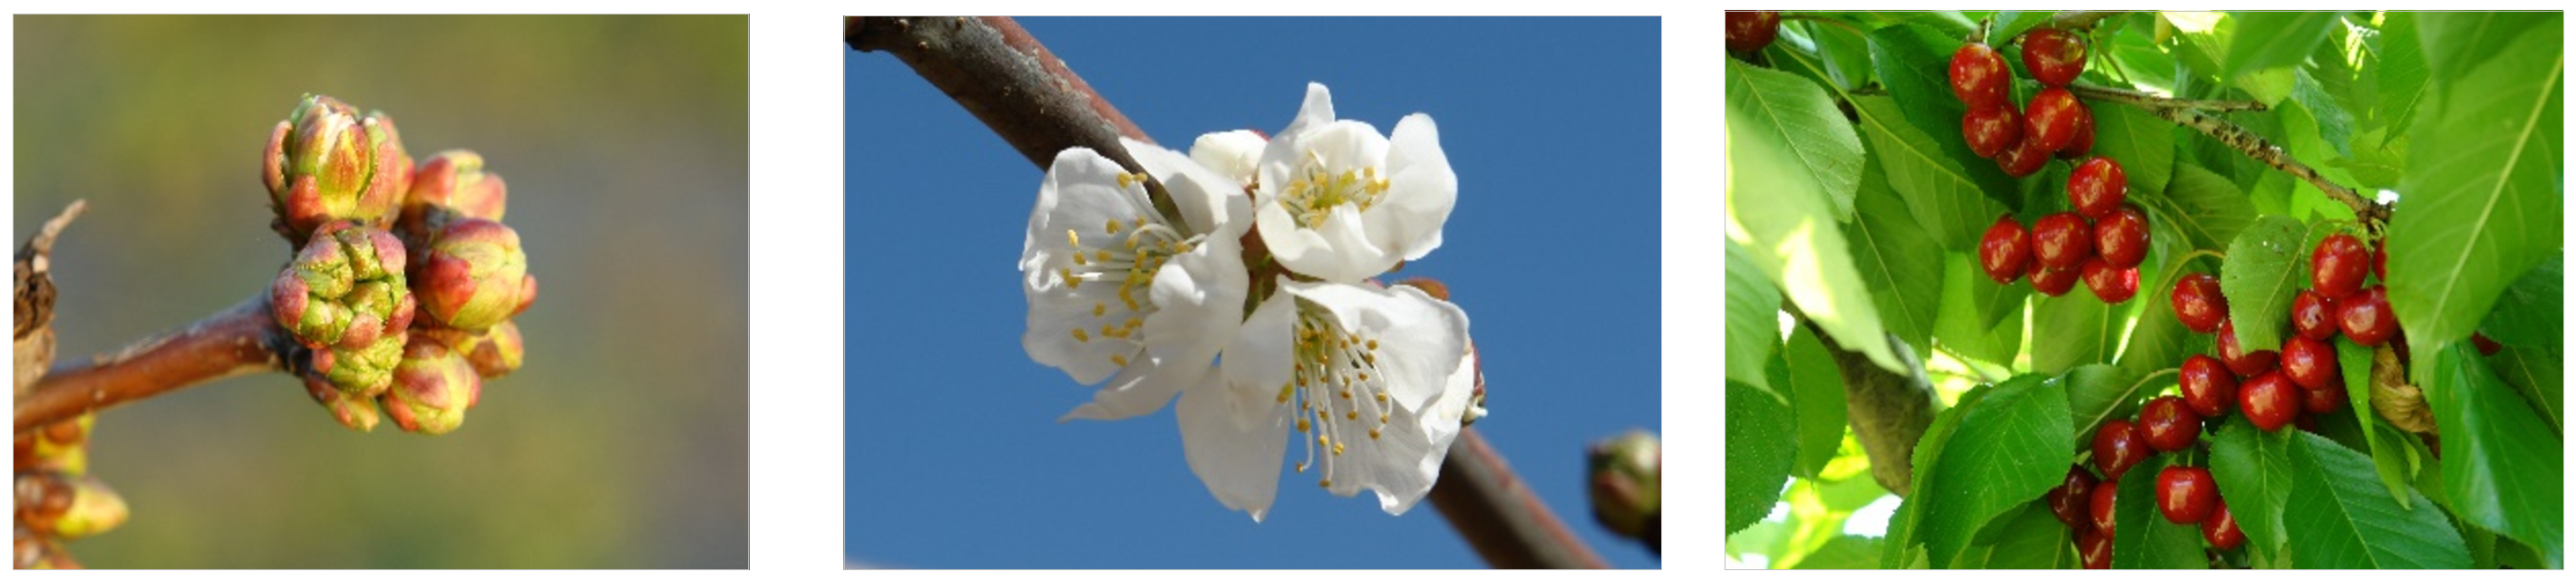
\includegraphics{./pheno_stages.png}
\caption{Picture 1 BBCH =55; Picture 2 BBCH =67; Picture 3 BBCH =89}
\end{figure}

\hypertarget{climate-change-and-impact-projection}{%
\chapter{Climate change and impact projection}\label{climate-change-and-impact-projection}}

\hypertarget{task-1-1}{%
\section{Task 1}\label{task-1-1}}

\textbf{List the main drivers of climate change at the decade to century scale, and briefly explain the mechanism through which the currently most important driver affects our climate}

\begin{table}

\caption{\label{tab:unnamed-chunk-2}Drivers of Climate Change}
\centering
\begin{tabular}[t]{l}
\hline
Drivers of climate change\\
\hline
Sun\\
\hline
Aerosols\\
\hline
Clouds\\
\hline
Ozone\\
\hline
Surface albedo\\
\hline
Greenhouse gases\\
\hline
\end{tabular}
\end{table}

\begin{quote}
The most important factor that currently has the greatest influence on climate and climate change is greenhouse gases. The most important greenhouse gases are water vapor, (carbon dioxide) CO2, (methane) CH4, and (nitrous oxides) N2O. Greenhouse gases can only absorb radiation of certain wavelengths. They absorb radiation with long wavelengths, which comes from the Earth's surface in the form of infrared radiation emitted by the warm Earth's surface. This radiation cannot leave the atmosphere and is trapped by the greenhouse gases, which returns it back to the Earth.
\end{quote}

\hypertarget{task-2-1}{%
\section{Task 2}\label{task-2-1}}

\textbf{Explain briefly what is special about temperature dynamics of the recent decades, and why we have good reasons to be concerned}

\begin{quote}
Over the past decades and throughout the last century, the temperature has been rising worldwide. Initially, this increase was relatively slow. The ten warmest years worldwide since 1880 were all measured after the millennium. The five warmest years worldwide were all recorded after 2014. This effect is also noticeable in Germany. Here, too, the ten warmest years were all measured after 2000, with one exception. If one places the temperature increase of the last decades in the climate history of the last one million years, it can be seen that there has never been such a strong temperature increase over such a relatively short period of time.

This rapid rise in temperature is developing its own dynamic. For example, high temperatures in the tundra cause the permafrost to thaw, releasing a large amount of CO2, a greenhouse gas that promotes even faster warming.
\end{quote}

\hypertarget{manual-chill-analysis}{%
\chapter{Manual Chill Analysis}\label{manual-chill-analysis}}

\begin{quote}
The \texttt{Winters\_hours\_gaps} data set has the columns: \texttt{Year}, \texttt{Month}, \texttt{Day}, \texttt{Hour}, \texttt{Temp\_gaps}, \texttt{Temp}. First, the function \texttt{cleaned\_data} is used to remove unnecessary columns such as \texttt{Temp\_gaps()} from the data set.
\end{quote}

\begin{Shaded}
\begin{Highlighting}[]
\CommentTok{#Clean Function}
\NormalTok{cleaned_data =}\StringTok{ }\ControlFlowTok{function}\NormalTok{(data_source) \{}
\NormalTok{  data_source =}\StringTok{ }
\StringTok{    }\NormalTok{data_source[, }\KeywordTok{c}\NormalTok{(}\StringTok{"Year"}\NormalTok{, }\StringTok{"Month"}\NormalTok{, }\StringTok{"Day"}\NormalTok{, }\StringTok{"Hour"}\NormalTok{, }\StringTok{"Temp"}\NormalTok{)]}
  \KeywordTok{return}\NormalTok{(data_source)}
\NormalTok{\}}

\CommentTok{# Apply Function to Winters_hours_gaps}
\KeywordTok{kable}\NormalTok{(}\KeywordTok{head}\NormalTok{(}\KeywordTok{cleaned_data}\NormalTok{(}\DataTypeTok{data_source =}\NormalTok{ Winters_hours_gaps)),}
      \DataTypeTok{caption =} \StringTok{"Cleaned  Dataset: Winters_hours_gaps"}\NormalTok{)}\OperatorTok
\StringTok{      }\KeywordTok{kable_styling}\NormalTok{(}\StringTok{"striped"}\NormalTok{, }\DataTypeTok{position =} \StringTok{"left"}\NormalTok{, }\DataTypeTok{font_size =} \DecValTok{10}\NormalTok{)}\OperatorTok
\StringTok{      }\KeywordTok{scroll_box}\NormalTok{(}\DataTypeTok{width =} \StringTok{"100%"}\NormalTok{)}
\end{Highlighting}
\end{Shaded}

\textbackslash begin\{table\}

\textbackslash caption\{\label{tab:unnamed-chunk-4}Cleaned Dataset: Winters\_hours\_gaps\}
\fontsize{10}{12}\selectfont

\begin{tabular}[t]{r|r|r|r|r}
\hline
Year & Month & Day & Hour & Temp\\
\hline
2008 & 3 & 3 & 10 & 15.127\\
\hline
2008 & 3 & 3 & 11 & 17.153\\
\hline
2008 & 3 & 3 & 12 & 18.699\\
\hline
2008 & 3 & 3 & 13 & 18.699\\
\hline
2008 & 3 & 3 & 14 & 18.842\\
\hline
2008 & 3 & 3 & 15 & 19.508\\
\hline
\end{tabular}

\textbackslash end\{table\}

\hypertarget{task-1-2}{%
\section{Task 1}\label{task-1-2}}

\textbf{Write a basic function that calculates warm hours (\textgreater25°C)}

\begin{Shaded}
\begin{Highlighting}[]
\NormalTok{WH =}\StringTok{ }\ControlFlowTok{function}\NormalTok{(hourtemps)}
\NormalTok{\{}
\NormalTok{  hourtemps[, }\StringTok{"warm_hours"}\NormalTok{] <-}\StringTok{ }\NormalTok{hourtemps}\OperatorTok{$}\NormalTok{Temp }\OperatorTok{>=}\StringTok{ }\FloatTok{25.0}
  \KeywordTok{return}\NormalTok{(hourtemps)}
\NormalTok{\}}
\end{Highlighting}
\end{Shaded}

\hypertarget{task-2-2}{%
\section{Task 2}\label{task-2-2}}

\textbf{Apply this function to the Winters\_hours\_gaps dataset}

\begin{Shaded}
\begin{Highlighting}[]
\CommentTok{# have a look to the data set}
\KeywordTok{kable}\NormalTok{(}\KeywordTok{head}\NormalTok{(Winters_hours_gaps),}\DataTypeTok{caption =} 
        \StringTok{"Example Dataset: Winters_hours_gaps"}\NormalTok{)}\OperatorTok
\StringTok{        }\KeywordTok{kable_styling}\NormalTok{(}\StringTok{"striped"}\NormalTok{, }\DataTypeTok{position =} \StringTok{"left"}\NormalTok{, }\DataTypeTok{font_size =} \DecValTok{10}\NormalTok{)}\OperatorTok
\StringTok{        }\KeywordTok{scroll_box}\NormalTok{(}\DataTypeTok{width =} \StringTok{"100%"}\NormalTok{)}
\end{Highlighting}
\end{Shaded}

\textbackslash begin\{table\}

\textbackslash caption\{\label{tab:unnamed-chunk-6}Example Dataset: Winters\_hours\_gaps\}
\fontsize{10}{12}\selectfont

\begin{tabular}[t]{r|r|r|r|r|r}
\hline
Year & Month & Day & Hour & Temp\_gaps & Temp\\
\hline
2008 & 3 & 3 & 10 & 15.127 & 15.127\\
\hline
2008 & 3 & 3 & 11 & 17.153 & 17.153\\
\hline
2008 & 3 & 3 & 12 & 18.699 & 18.699\\
\hline
2008 & 3 & 3 & 13 & 18.699 & 18.699\\
\hline
2008 & 3 & 3 & 14 & 18.842 & 18.842\\
\hline
2008 & 3 & 3 & 15 & 19.508 & 19.508\\
\hline
\end{tabular}

\textbackslash end\{table\}

\begin{Shaded}
\begin{Highlighting}[]
\CommentTok{# Apply Function}
\NormalTok{hourtemps =}\StringTok{ }\KeywordTok{cleaned_data}\NormalTok{(}\DataTypeTok{data_source =}\NormalTok{ Winters_hours_gaps)}
\KeywordTok{kable}\NormalTok{(}\KeywordTok{head}\NormalTok{(}\KeywordTok{WH}\NormalTok{(}\DataTypeTok{hourtemps =}\NormalTok{ hourtemps)))}\OperatorTok
\StringTok{        }\KeywordTok{kable_styling}\NormalTok{(}\StringTok{"striped"}\NormalTok{, }\DataTypeTok{position =} \StringTok{"left"}\NormalTok{, }\DataTypeTok{font_size =} \DecValTok{10}\NormalTok{)}\OperatorTok
\StringTok{        }\KeywordTok{scroll_box}\NormalTok{(}\DataTypeTok{width =} \StringTok{"100%"}\NormalTok{)}
\end{Highlighting}
\end{Shaded}

\begingroup\fontsize{10}{12}\selectfont

\begin{tabular}{r|r|r|r|r|l}
\hline
Year & Month & Day & Hour & Temp & warm\_hours\\
\hline
2008 & 3 & 3 & 10 & 15.127 & FALSE\\
\hline
2008 & 3 & 3 & 11 & 17.153 & FALSE\\
\hline
2008 & 3 & 3 & 12 & 18.699 & FALSE\\
\hline
2008 & 3 & 3 & 13 & 18.699 & FALSE\\
\hline
2008 & 3 & 3 & 14 & 18.842 & FALSE\\
\hline
2008 & 3 & 3 & 15 & 19.508 & FALSE\\
\hline
\end{tabular}
\endgroup{}

\hypertarget{task-3-1}{%
\section{Task 3}\label{task-3-1}}

\textbf{Extend this function, so that it can take start and end dates as inputs and sums up warm hours between these dates}

\begin{Shaded}
\begin{Highlighting}[]
\NormalTok{warm_hours_function =}\StringTok{ }\ControlFlowTok{function}\NormalTok{(Input_Data,}
\NormalTok{                               S_Jahr,}
\NormalTok{                               S_Monat,}
\NormalTok{                               S_Tag,}
\NormalTok{                               S_Stunde,}
\NormalTok{                               E_Jahr,}
\NormalTok{                               E_Monat,}
\NormalTok{                               E_Tag,}
\NormalTok{                               E_Stunde) \{}
\NormalTok{  Start_Date <-}
\StringTok{    }\KeywordTok{which}\NormalTok{(}
\NormalTok{      hourtemps}\OperatorTok{$}\NormalTok{Year }\OperatorTok{==}\StringTok{ }\NormalTok{S_Jahr }\OperatorTok{&}\StringTok{ }\NormalTok{hourtemps}\OperatorTok{$}\NormalTok{Month }\OperatorTok{==}\StringTok{ }\NormalTok{S_Monat }\OperatorTok{&}
\StringTok{        }\NormalTok{hourtemps}\OperatorTok{$}\NormalTok{Day }\OperatorTok{==}\StringTok{ }\NormalTok{S_Tag }\OperatorTok{&}
\StringTok{        }\NormalTok{hourtemps}\OperatorTok{$}\NormalTok{Hour }\OperatorTok{==}\StringTok{ }\NormalTok{S_Stunde}
\NormalTok{    )}
\NormalTok{  End_Date <-}\StringTok{ }\KeywordTok{which}\NormalTok{(}
\NormalTok{    hourtemps}\OperatorTok{$}\NormalTok{Year }\OperatorTok{==}\StringTok{ }\NormalTok{E_Jahr }\OperatorTok{&}\StringTok{ }\NormalTok{hourtemps}\OperatorTok{$}\NormalTok{Month }\OperatorTok{==}\StringTok{ }\NormalTok{E_Monat }\OperatorTok{&}
\StringTok{      }\NormalTok{hourtemps}\OperatorTok{$}\NormalTok{Day }\OperatorTok{==}\StringTok{ }\NormalTok{E_Tag }\OperatorTok{&}\StringTok{ }\NormalTok{hourtemps}\OperatorTok{$}\NormalTok{Hour }\OperatorTok{==}\StringTok{ }\NormalTok{E_Stunde}
\NormalTok{  )}
  
  \CommentTok{# Apply Function Warm Hours (WH)}
\NormalTok{  hourtemps =}\StringTok{ }\KeywordTok{WH}\NormalTok{(}\DataTypeTok{hourtemps =}\NormalTok{ Input_Data)}
  
  \CommentTok{# Calculate warm_hours}
\NormalTok{  warm_hours =}\StringTok{ }\KeywordTok{sum}\NormalTok{(hourtemps}\OperatorTok{$}\NormalTok{warm_hours[Start_Date}\OperatorTok{:}\NormalTok{End_Date])}
  
  \KeywordTok{return}\NormalTok{(}\KeywordTok{cat}\NormalTok{(}\StringTok{"The number of heat hours is:"}\NormalTok{, }\KeywordTok{paste}\NormalTok{(warm_hours)))}
\NormalTok{\}}

\KeywordTok{warm_hours_function}\NormalTok{(}
  \DataTypeTok{Input_Data =}\NormalTok{ hourtemps,}
  \DataTypeTok{S_Jahr =} \DecValTok{2008}\NormalTok{,}
  \DataTypeTok{S_Monat =} \DecValTok{5}\NormalTok{,}
  \DataTypeTok{S_Tag =} \DecValTok{1}\NormalTok{,}
  \DataTypeTok{S_Stunde =} \DecValTok{12}\NormalTok{,}
  \DataTypeTok{E_Jahr =} \DecValTok{2008}\NormalTok{,}
  \DataTypeTok{E_Monat =} \DecValTok{8}\NormalTok{,}
  \DataTypeTok{E_Tag =} \DecValTok{31}\NormalTok{,}
  \DataTypeTok{E_Stunde =} \DecValTok{12}
\NormalTok{)}
\end{Highlighting}
\end{Shaded}

\begin{verbatim}
## The number of heat hours is: 957
\end{verbatim}

\hypertarget{chill-models}{%
\chapter{Chill Models}\label{chill-models}}

\begin{quote}
Counting chill hours can be done in various ways. \texttt{ChillR} offers some functions for this purpose. The simplest function for this is the \texttt{Chilling\_Hours()} function. It records one chill hour for every temperature between 0 and 7.2 degrees.
A slightly more complex function is the \texttt{Utah\_Model()} function. It evaluates the measured temperatures and decides whether a full chill hour was reached or only half. For example, if the temperature is between 1 and 2 degrees, one chill hour has been reached. If it is between 3 and 4 degrees, two chill hours are recorded.
The \texttt{Dynamic\_model()} function is the most complex function. It is taken from an Excel sheet.
The \texttt{chilling()} function combines the functions described above and presents the results in an overview.
\end{quote}

\hypertarget{task-1-3}{%
\section{Task 1}\label{task-1-3}}

\textbf{Run the chilling() function on the Winters\_hours\_gap dataset}

\begin{Shaded}
\begin{Highlighting}[]
\CommentTok{# run chilling function on Winters_hours_gap dataset}
\NormalTok{output =}
\StringTok{  }\KeywordTok{chilling}\NormalTok{(}\KeywordTok{make_JDay}\NormalTok{(Winters_hours_gaps),}
           \DataTypeTok{Start_JDay =} \DecValTok{90}\NormalTok{,}
           \DataTypeTok{End_JDay =} \DecValTok{100}\NormalTok{)}

\KeywordTok{kable}\NormalTok{(output, }\DataTypeTok{caption =}\StringTok{"chilling function on Winters_hours_gap"}\NormalTok{) }\OperatorTok
\StringTok{        }\KeywordTok{kable_styling}\NormalTok{(}\StringTok{"striped"}\NormalTok{, }\DataTypeTok{position =} \StringTok{"left"}\NormalTok{, }\DataTypeTok{font_size =} \DecValTok{10}\NormalTok{)}\OperatorTok
\StringTok{        }\KeywordTok{scroll_box}\NormalTok{(}\DataTypeTok{width =} \StringTok{"100%"}\NormalTok{)}
\end{Highlighting}
\end{Shaded}

\textbackslash begin\{table\}

\textbackslash caption\{\label{tab:unnamed-chunk-9}chilling function on Winters\_hours\_gap\}
\fontsize{10}{12}\selectfont

\begin{tabular}[t]{l|r|r|r|r|r|r|r|r}
\hline
Season & End\_year & Season\_days & Data\_days & Perc\_complete & Chilling\_Hours & Utah\_Model & Chill\_portions & GDH\\
\hline
2007/2008 & 2008 & 11 & 11 & 100 & 40 & 15.5 & 2.009147 & 2406.52\\
\hline
\end{tabular}

\textbackslash end\{table\}

\hypertarget{task2}{%
\section{Task2}\label{task2}}

\textbf{Create your own temperature-weighting chill model using the \texttt{step\_model()} function}

\begin{quote}
The \texttt{step\_model} function has two arguments that the user can pass. One is a dataset of temperature data \texttt{HourTemp} and the other is a \texttt{data.frame()} (df) consisting of \texttt{lower}, \texttt{upper}, and \texttt{weight}. A pre-defined lower temperature range from, for example, -1000 °C to 0 °C is set, with all temperatures within this range being assigned a weight of 0. Assuming that hourly temperature data is provided as input, the
temperature can be multiplied by the corresponding weight to obtain the amount of ``chillhours''. For example: -1 °C is within the range {[}-1000, 0{]} == 0, resulting in 0 chillhours. Another argument is \texttt{summ}. If \texttt{summ\ =\ TRUE}, the cumulative chillhours over a defined period will be output. If \texttt{summ\ =\ FALSE}, the weights of the chillhours will be output.
\end{quote}

\begin{Shaded}
\begin{Highlighting}[]
\NormalTok{step_model =}\StringTok{ }\ControlFlowTok{function}\NormalTok{ (HourTemp,}
                        \DataTypeTok{df =}
                          \KeywordTok{data.frame}\NormalTok{(}
                            \DataTypeTok{lower =} \KeywordTok{c}\NormalTok{(}\OperatorTok{-}\DecValTok{1000}\NormalTok{, }\FloatTok{1.4}\NormalTok{, }\FloatTok{2.4}\NormalTok{, }\FloatTok{9.1}\NormalTok{, }\FloatTok{12.4}\NormalTok{, }\FloatTok{15.9}\NormalTok{, }\DecValTok{18}\NormalTok{),}
                            \DataTypeTok{upper =} \KeywordTok{c}\NormalTok{(}\FloatTok{1.4}\NormalTok{, }\FloatTok{2.4}\NormalTok{, }\FloatTok{9.1}\NormalTok{, }\FloatTok{12.4}\NormalTok{, }\FloatTok{15.9}\NormalTok{, }\DecValTok{18}\NormalTok{, }\DecValTok{1000}\NormalTok{),}
                            \DataTypeTok{weight =} \KeywordTok{c}\NormalTok{(}\DecValTok{0}\NormalTok{, }\FloatTok{0.5}\NormalTok{, }\DecValTok{1}\NormalTok{, }\FloatTok{0.5}\NormalTok{, }\DecValTok{0}\NormalTok{, }\FloatTok{-0.5}\NormalTok{, }\DecValTok{-1}\NormalTok{)}
\NormalTok{                          ),}
                        \DataTypeTok{summ =} \OtherTok{TRUE}\NormalTok{)}
\NormalTok{\{}
\NormalTok{  lower <-}\StringTok{ }\NormalTok{df}\OperatorTok{$}\NormalTok{lower}
\NormalTok{  upper <-}\StringTok{ }\NormalTok{df}\OperatorTok{$}\NormalTok{upper}
\NormalTok{  weight <-}\StringTok{ }\NormalTok{df}\OperatorTok{$}\NormalTok{weight}
  \ControlFlowTok{if}\NormalTok{ (summ }\OperatorTok{==}\StringTok{ }\OtherTok{TRUE}\NormalTok{)}
    \KeywordTok{return}\NormalTok{(}\KeywordTok{cumsum}\NormalTok{(}\KeywordTok{sapply}\NormalTok{(HourTemp, }\ControlFlowTok{function}\NormalTok{(x)}
\NormalTok{      weight[}\KeywordTok{which}\NormalTok{(x }\OperatorTok{>}
\StringTok{                     }\NormalTok{lower }\OperatorTok{&}\StringTok{ }\NormalTok{x }\OperatorTok{<=}\StringTok{ }\NormalTok{upper)])))}
  \ControlFlowTok{else}
    \KeywordTok{return}\NormalTok{(}\KeywordTok{sapply}\NormalTok{(HourTemp, }\ControlFlowTok{function}\NormalTok{(x)}
\NormalTok{      weight[}\KeywordTok{which}\NormalTok{(x }\OperatorTok{>}
\StringTok{                     }\NormalTok{lower }\OperatorTok{&}\StringTok{ }\NormalTok{x }\OperatorTok{<=}\StringTok{ }\NormalTok{upper)]))}
\NormalTok{\}}
\end{Highlighting}
\end{Shaded}

\begin{quote}
Here, only an ``own data field'' is defined with its own limits that have their own weight. For example, from -100 °C to 0 °C, the weight is set to 0. In this case, no ``chillhour'' occurs. If the temperature is between 0 °C and 2 °C, the weight of the ``chillhour'' is 0.5. In this case, half a ``chillhour'' occurs.
\end{quote}

\begin{Shaded}
\begin{Highlighting}[]
\NormalTok{own_df =}\StringTok{ }\KeywordTok{data.frame}\NormalTok{ (}\DataTypeTok{lower  =} \KeywordTok{c}\NormalTok{(}\OperatorTok{-}\DecValTok{100}\NormalTok{,}\DecValTok{0}\NormalTok{,  }\DecValTok{2}\NormalTok{, }\DecValTok{4}\NormalTok{,  }\DecValTok{5}\NormalTok{, }\DecValTok{6}\NormalTok{,   }\DecValTok{7}\NormalTok{    ),}
                     \DataTypeTok{upper  =} \KeywordTok{c}\NormalTok{(  }\DecValTok{0}\NormalTok{, }\DecValTok{2}\NormalTok{,  }\DecValTok{4}\NormalTok{, }\DecValTok{5}\NormalTok{,  }\DecValTok{6}\NormalTok{, }\DecValTok{7}\NormalTok{,   }\DecValTok{100}\NormalTok{  ),}
                     \DataTypeTok{weight =} \KeywordTok{c}\NormalTok{(  }\DecValTok{0}\NormalTok{, }\FloatTok{0.5}\NormalTok{,}\DecValTok{1}\NormalTok{, }\FloatTok{1.5}\NormalTok{,}\DecValTok{1}\NormalTok{, }\FloatTok{0.5}\NormalTok{, }\DecValTok{0}\NormalTok{    ))}
\end{Highlighting}
\end{Shaded}

\begin{quote}
After the dataframe with your own weights has been created, it can be implemented into the \texttt{step\_model()} function.
\end{quote}

\begin{Shaded}
\begin{Highlighting}[]
\NormalTok{use_step_model =}\StringTok{ }\ControlFlowTok{function}\NormalTok{(x)\{}\KeywordTok{step_model}\NormalTok{(x,own_df)\}}
  
\CommentTok{# quick aplly }
\KeywordTok{use_step_model}\NormalTok{(}\DataTypeTok{x =}\NormalTok{ Winters_hours_gaps}\OperatorTok{$}\NormalTok{Temp)[}\DecValTok{1}\OperatorTok{:}\DecValTok{100}\NormalTok{]}
\end{Highlighting}
\end{Shaded}

\begin{verbatim}
##   [1]  0.0  0.0  0.0  0.0  0.0  0.0  0.0  0.0  0.0  0.0  0.0  0.0  0.0  0.0  0.5
##  [16]  1.0  1.0  1.0  1.5  2.5  3.5  4.5  4.5  4.5  4.5  4.5  4.5  4.5  4.5  4.5
##  [31]  4.5  4.5  4.5  4.5  4.5  4.5  4.5  4.5  4.5  4.5  4.5  4.5  4.5  4.5  4.5
##  [46]  4.5  4.5  4.5  4.5  4.5  4.5  4.5  4.5  4.5  4.5  4.5  4.5  4.5  4.5  4.5
##  [61]  4.5  5.0  5.5  6.0  7.0  8.5  9.5 10.5 11.5 12.5 13.0 13.0 13.0 13.0 13.0
##  [76] 13.0 13.0 13.0 13.0 13.0 13.0 13.0 13.0 13.0 13.0 13.5 14.0 15.0 16.5 18.0
##  [91] 19.5 21.0 22.0 23.0 23.0 23.0 23.0 23.0 23.0 23.0
\end{verbatim}

\hypertarget{task3}{%
\section{Task3}\label{task3}}

\textbf{Run this model on the Winters\_hours\_gaps dataset using the tempResponse() function}

\begin{quote}
The \texttt{tempResponse()} function can display and summarize some chill models. Here is the model \texttt{weather\_mill()} our own chilling model which is created by the \texttt{step\_model()}. The modified \texttt{step\_model()} function is renamed to \texttt{use\_step\_model()} and passed as a parameter to the tempResponse function (weather\_mill = use\_step\_model).
\end{quote}

\begin{Shaded}
\begin{Highlighting}[]
\NormalTok{output <-}
\StringTok{  }\KeywordTok{tempResponse}\NormalTok{(}
    \KeywordTok{make_JDay}\NormalTok{(Winters_hours_gaps),}
    \DataTypeTok{Start_JDay =} \DecValTok{30}\NormalTok{,}
    \DataTypeTok{End_JDay =} \DecValTok{100}\NormalTok{,}
    \DataTypeTok{models =} \KeywordTok{list}\NormalTok{(}
      \DataTypeTok{Chill_Portions =}\NormalTok{ Dynamic_Model,}
      \DataTypeTok{GDH =}\NormalTok{ GDH,}
      \DataTypeTok{weather_mill =}\NormalTok{ use_step_model, }\CommentTok{# own model weather_mill}
      \DataTypeTok{Utah_Model =}\NormalTok{ Utah_Model}
\NormalTok{    )}
\NormalTok{  )}

\CommentTok{# display result}
\KeywordTok{kable}\NormalTok{(output, }\DataTypeTok{caption =} \StringTok{"Summarized some models"}\NormalTok{) }\OperatorTok
\StringTok{        }\KeywordTok{kable_styling}\NormalTok{(}\StringTok{"striped"}\NormalTok{, }\DataTypeTok{position =} \StringTok{"left"}\NormalTok{, }\DataTypeTok{font_size =} \DecValTok{10}\NormalTok{)}\OperatorTok
\StringTok{        }\KeywordTok{scroll_box}\NormalTok{(}\DataTypeTok{width =} \StringTok{"100%"}\NormalTok{)}
\end{Highlighting}
\end{Shaded}

\begin{table}

\caption{\label{tab:unnamed-chunk-13}Summarized some models}
\fontsize{10}{12}\selectfont
\begin{tabular}[t]{l|r|r|r|r|r|r|r|r}
\hline
Season & End\_year & Season\_days & Data\_days & Perc\_complete & Chill\_Portions & GDH & weather\_mill & Utah\_Model\\
\hline
2007/2008 & 2008 & 71 & 37.58333 & 52.93427 & 5.930439 & 8392.585 & 84 & 49.5\\
\hline
\end{tabular}
\end{table}

\begin{quote}
If the Utah Model is included, which is based on the default settings of the Step Model, a clear difference between the modified Step Model and the Utah Model can be observed.
\end{quote}

\hypertarget{making-hourly-temperatures}{%
\chapter{Making hourly temperatures}\label{making-hourly-temperatures}}

\hypertarget{task-1-4}{%
\section{Task 1}\label{task-1-4}}

\textbf{Choose a location of interest, find out its latitude and produce plots of daily sunrise, sunset and daylength}

\begin{quote}
First, I would like to compare the lengths of days among locations of interest. I have selected Glogau in Poland, Zülpich in Germany, Tenerife in Spain, Moscow in Russia, and Karkaralinsk in Kazakhstan.
\end{quote}

\begin{Shaded}
\begin{Highlighting}[]
\CommentTok{# initialize the variables with daylength, sunrise and sunset by the function daylength}
\NormalTok{Glogau      <-}\StringTok{ }\KeywordTok{daylength}\NormalTok{(}\DataTypeTok{latitude =} \FloatTok{51.40}\NormalTok{, }\DataTypeTok{JDay =} \DecValTok{1}\OperatorTok{:}\DecValTok{365}\NormalTok{)}
\NormalTok{Teneriffa   <-}\StringTok{ }\KeywordTok{daylength}\NormalTok{(}\DataTypeTok{latitude =} \FloatTok{28.19}\NormalTok{, }\DataTypeTok{JDay =} \DecValTok{1}\OperatorTok{:}\DecValTok{365}\NormalTok{)}
\NormalTok{Zuelpich    <-}\StringTok{ }\KeywordTok{daylength}\NormalTok{(}\DataTypeTok{latitude =} \FloatTok{50.42}\NormalTok{, }\DataTypeTok{JDay =} \DecValTok{1}\OperatorTok{:}\DecValTok{365}\NormalTok{)}
\NormalTok{Moskau      <-}\StringTok{ }\KeywordTok{daylength}\NormalTok{(}\DataTypeTok{latitude =} \FloatTok{55.45}\NormalTok{, }\DataTypeTok{JDay =} \DecValTok{1}\OperatorTok{:}\DecValTok{365}\NormalTok{)}
\NormalTok{Karkaralinsk <-}\StringTok{ }\KeywordTok{daylength}\NormalTok{(}\DataTypeTok{latitude =} \FloatTok{49.24}\NormalTok{, }\DataTypeTok{JDay =} \DecValTok{1}\OperatorTok{:}\DecValTok{365}\NormalTok{)}

\CommentTok{# Create a dataframe consisting of the variables "base" (days 1 to 365) and the}
\CommentTok{# respective locations and containing only the day length for each location.}
\NormalTok{df <-}\StringTok{ }\KeywordTok{data.frame}\NormalTok{(}
  \DataTypeTok{base         =} \KeywordTok{seq}\NormalTok{(}\KeywordTok{length}\NormalTok{(Glogau[[}\DecValTok{1}\NormalTok{]])),}
  \DataTypeTok{Glogau       =}\NormalTok{ Glogau[[}\DecValTok{3}\NormalTok{]],}
  \DataTypeTok{Teneriffa    =}\NormalTok{ Teneriffa[[}\DecValTok{3}\NormalTok{]],}
\NormalTok{  Zülpich      =}\StringTok{ }\NormalTok{Zuelpich[[}\DecValTok{3}\NormalTok{]],}
  \DataTypeTok{Moskau       =}\NormalTok{ Moskau[[}\DecValTok{3}\NormalTok{]],}
  \DataTypeTok{Karkaralinsk =}\NormalTok{ Karkaralinsk[[}\DecValTok{3}\NormalTok{]]}
\NormalTok{)}


\KeywordTok{kable}\NormalTok{(}\KeywordTok{head}\NormalTok{(df), }\DataTypeTok{caption =} \StringTok{"Differnt Locations"}\NormalTok{) }\OperatorTok\StringTok{ }
\StringTok{       }\KeywordTok{kable_styling}\NormalTok{(}\StringTok{"striped"}\NormalTok{, }\DataTypeTok{position =} \StringTok{"left"}\NormalTok{, }\DataTypeTok{font_size =} \DecValTok{10}\NormalTok{)}\OperatorTok
\StringTok{        }\KeywordTok{scroll_box}\NormalTok{(}\DataTypeTok{width =} \StringTok{"100%"}\NormalTok{)}
\end{Highlighting}
\end{Shaded}

\begin{table}

\caption{\label{tab:unnamed-chunk-14}Differnt Locations}
\fontsize{10}{12}\selectfont
\begin{tabular}[t]{r|r|r|r|r|r}
\hline
base & Glogau & Teneriffa & Zülpich & Moskau & Karkaralinsk\\
\hline
1 & 7.930050 & 10.38197 & 8.086864 & 7.175796 & 8.265160\\
\hline
2 & 7.948054 & 10.38872 & 8.104044 & 7.198073 & 8.281428\\
\hline
3 & 7.967737 & 10.39612 & 8.122830 & 7.222407 & 8.299217\\
\hline
4 & 7.989077 & 10.40415 & 8.143199 & 7.248768 & 8.318509\\
\hline
5 & 8.012048 & 10.41281 & 8.165129 & 7.277120 & 8.339282\\
\hline
6 & 8.036625 & 10.42209 & 8.188595 & 7.307424 & 8.361515\\
\hline
\end{tabular}
\end{table}

\begin{Shaded}
\begin{Highlighting}[]
\CommentTok{# create a pivot table}
\NormalTok{df_long <-}
\StringTok{  }\KeywordTok{pivot_longer}\NormalTok{(df, }\OperatorTok{-}\StringTok{"base"}\NormalTok{, }\DataTypeTok{names_to =} \StringTok{"Location"}\NormalTok{, }\DataTypeTok{values_to =} \StringTok{"daylength"}\NormalTok{)}

\KeywordTok{kable}\NormalTok{(}\KeywordTok{head}\NormalTok{(df_long)) }\OperatorTok\StringTok{ }
\StringTok{      }\KeywordTok{kable_styling}\NormalTok{(}\StringTok{"striped"}\NormalTok{, }\DataTypeTok{position =} \StringTok{"left"}\NormalTok{, }\DataTypeTok{font_size =} \DecValTok{10}\NormalTok{)}\OperatorTok
\StringTok{      }\KeywordTok{scroll_box}\NormalTok{(}\DataTypeTok{width =} \StringTok{"100%"}\NormalTok{)}
\end{Highlighting}
\end{Shaded}

\begingroup\fontsize{10}{12}\selectfont

\begin{tabular}{r|l|r}
\hline
base & Location & daylength\\
\hline
1 & Glogau & 7.930050\\
\hline
1 & Teneriffa & 10.381965\\
\hline
1 & Zülpich & 8.086864\\
\hline
1 & Moskau & 7.175796\\
\hline
1 & Karkaralinsk & 8.265160\\
\hline
2 & Glogau & 7.948054\\
\hline
\end{tabular}
\endgroup{}

\begin{Shaded}
\begin{Highlighting}[]
\CommentTok{# plot the result with ggplot}
\KeywordTok{ggplot}\NormalTok{(df_long, }\KeywordTok{aes}\NormalTok{(}\DataTypeTok{x =}\NormalTok{ base, }\DataTypeTok{y =}\NormalTok{ daylength, }\DataTypeTok{groupe =}\NormalTok{ Location)) }\OperatorTok{+}
\StringTok{  }\KeywordTok{geom_line}\NormalTok{(}\KeywordTok{aes}\NormalTok{(}\DataTypeTok{color =}\NormalTok{ Location), }\DataTypeTok{lwd =} \FloatTok{1.0}\NormalTok{) }\OperatorTok{+}
\StringTok{  }\KeywordTok{ggtitle}\NormalTok{(}\StringTok{"Different day lengths in different places"}\NormalTok{) }\OperatorTok{+}
\StringTok{  }\KeywordTok{labs}\NormalTok{(}\DataTypeTok{x =} \StringTok{"Days"}\NormalTok{, }\DataTypeTok{y =} \StringTok{"Daylength [h]"}\NormalTok{) }\OperatorTok{+}\StringTok{ }\KeywordTok{theme_gray}\NormalTok{(}\DataTypeTok{base_size =} \DecValTok{15}\NormalTok{)}
\end{Highlighting}
\end{Shaded}

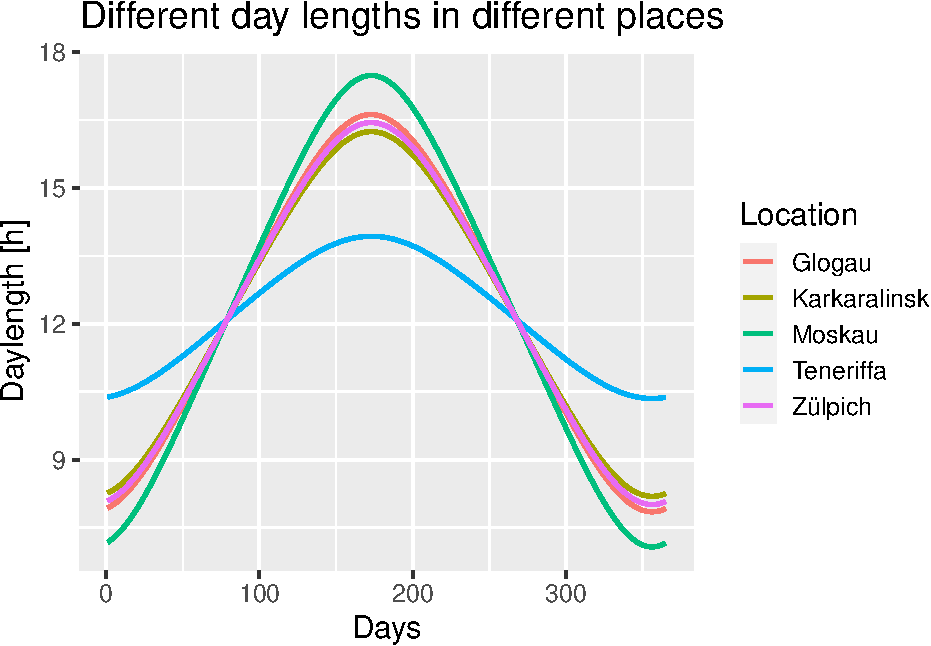
\includegraphics{Tree-Phenology_files/figure-latex/unnamed-chunk-14-1.pdf}

\begin{quote}
Create a summary of the sunrise, sunset, and day length for Moscow.
\end{quote}

\begin{Shaded}
\begin{Highlighting}[]
\NormalTok{Days <-}\StringTok{ }\KeywordTok{daylength}\NormalTok{(}\DataTypeTok{latitude =} \FloatTok{55.45}\NormalTok{, }\DataTypeTok{JDay =} \DecValTok{1}\OperatorTok{:}\DecValTok{365}\NormalTok{)}

\NormalTok{Days_df <-}
\StringTok{  }\KeywordTok{data.frame}\NormalTok{(}
    \DataTypeTok{JDay =} \DecValTok{1}\OperatorTok{:}\DecValTok{365}\NormalTok{,}
    \DataTypeTok{Sunrise =}\NormalTok{ Days}\OperatorTok{$}\NormalTok{Sunrise,}
    \DataTypeTok{Sunset =}\NormalTok{ Days}\OperatorTok{$}\NormalTok{Sunset,}
    \DataTypeTok{Daylength =}\NormalTok{ Days}\OperatorTok{$}\NormalTok{Daylength}
\NormalTok{  )}

\NormalTok{Days_df<-}\KeywordTok{melt}\NormalTok{(Days_df, }\DataTypeTok{id=}\KeywordTok{c}\NormalTok{(}\StringTok{"JDay"}\NormalTok{)) }
\end{Highlighting}
\end{Shaded}

\begin{quote}
Show the final result
\end{quote}

\begin{Shaded}
\begin{Highlighting}[]
\KeywordTok{ggplot}\NormalTok{(Days_df, }\KeywordTok{aes}\NormalTok{(}\DataTypeTok{x =}\NormalTok{ JDay, }\DataTypeTok{y =}\NormalTok{ value)) }\OperatorTok{+}\StringTok{ }\KeywordTok{geom_line}\NormalTok{(}\DataTypeTok{lwd =} \FloatTok{1.5}\NormalTok{, }\DataTypeTok{color =} \StringTok{"red"}\NormalTok{) }\OperatorTok{+}\StringTok{ }\KeywordTok{facet_grid}\NormalTok{(}\DataTypeTok{cols =} \KeywordTok{vars}\NormalTok{(variable)) }\OperatorTok{+}
\StringTok{  }\KeywordTok{ylab}\NormalTok{(}\StringTok{"Time of Day / Daylength (Hours)"}\NormalTok{) }\OperatorTok{+}\StringTok{ }\KeywordTok{theme_bw}\NormalTok{(}\DataTypeTok{base_size =} \DecValTok{20}\NormalTok{) }\OperatorTok{+}
\StringTok{  }\KeywordTok{ggtitle}\NormalTok{(}\StringTok{"Sunrise, Sunset and Daylength of Moskau"}\NormalTok{)}
\end{Highlighting}
\end{Shaded}

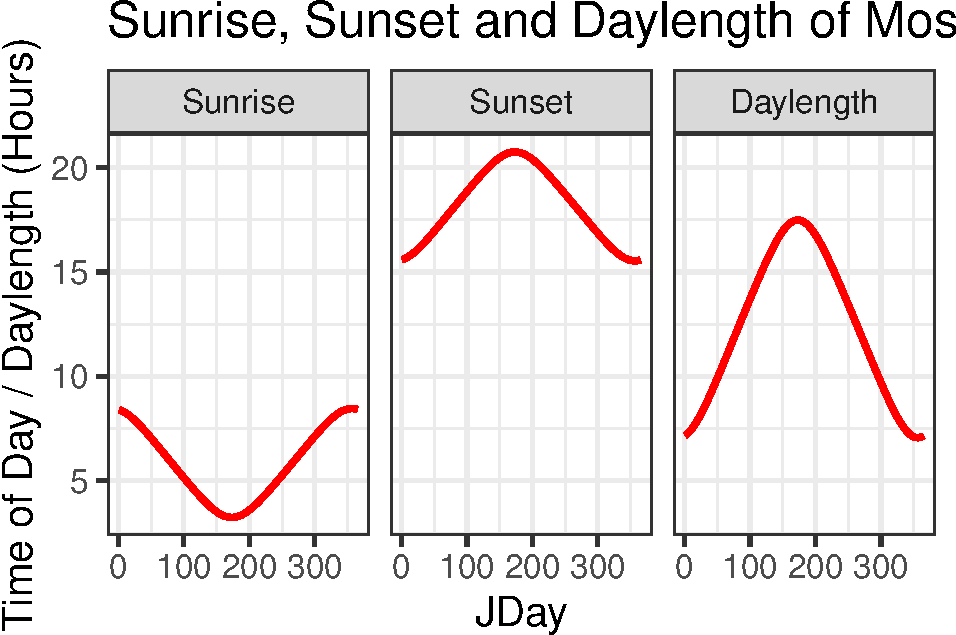
\includegraphics[width=0.8\linewidth]{Tree-Phenology_files/figure-latex/unnamed-chunk-16-1}

\hypertarget{task-2-3}{%
\section{Task 2}\label{task-2-3}}

\textbf{Produce an hourly dataset, based on idealized daily curves, for the KA\_weather dataset (included in chillR)}

\begin{quote}
The following two tasks were performed in a modified form. In order to demonstrate the application of the chillR package, it was decided to use a currently active weather station and use its data as a basis. Data on the weather station can be found in the table below.
\end{quote}

\begin{table}

\caption{\label{tab:unnamed-chunk-17}Weather Station Fuessenich}
\fontsize{10}{12}\selectfont
\begin{tabular}[t]{l|l|l|l}
\hline
Location & State & GPS & Gauß\_Krüger\\
\hline
Zuelpich - Fuessenich & North Rhine-Westphalia & 50.69527026369208, 6.615666577711913 & Rechtswert:2543500 Hochwert: 5617798\\
\hline
\end{tabular}
\end{table}

First, corresponding data must be read in. The data are already prepared.

\begin{Shaded}
\begin{Highlighting}[]
\NormalTok{Zuelpich_hourly =}\StringTok{ }\KeywordTok{read.table}\NormalTok{(}
  \StringTok{"weather_data/Weather_Zuelpich_2019_hourly.csv"}\NormalTok{,}
  \DataTypeTok{header =} \OtherTok{TRUE}\NormalTok{,}
  \DataTypeTok{sep =} \StringTok{","}
\NormalTok{)}

\NormalTok{Zuelpich_min_max =}\StringTok{ }\KeywordTok{read.table}\NormalTok{(}\StringTok{"weather_data/Weather_Zuelpich_2019.csv"}\NormalTok{,}
                              \DataTypeTok{header =} \OtherTok{TRUE}\NormalTok{,}
                              \DataTypeTok{sep =} \StringTok{","}\NormalTok{)}
\end{Highlighting}
\end{Shaded}

\begin{Shaded}
\begin{Highlighting}[]
\NormalTok{zuelpich_april =}\StringTok{ }\NormalTok{Zuelpich_hourly }\OperatorTok\StringTok{ }\KeywordTok{filter}\NormalTok{(}\StringTok{"2019-04-01 00:00:00"} \OperatorTok{<}\StringTok{ }\NormalTok{date) }\OperatorTok
\StringTok{  }\KeywordTok{filter}\NormalTok{(}\StringTok{"2019-04-05 00:00:00"} \OperatorTok{>}\StringTok{ }\NormalTok{date)}

\NormalTok{zuelpich_april}\OperatorTok{$}\NormalTok{date_new <-}\StringTok{ }\KeywordTok{as.POSIXct}\NormalTok{(zuelpich_april[, }\DecValTok{3}\NormalTok{])}
\NormalTok{zuelpich_april}\OperatorTok{$}\NormalTok{date_newnew =}\StringTok{ }\KeywordTok{as.Date}\NormalTok{(zuelpich_april[, }\DecValTok{3}\NormalTok{])}

\KeywordTok{kable}\NormalTok{(}\KeywordTok{head}\NormalTok{(zuelpich_april), }\DataTypeTok{caption =} \StringTok{"Dataset: zuelpich_april"}\NormalTok{) }\OperatorTok
\StringTok{        }\KeywordTok{kable_styling}\NormalTok{(}\StringTok{"striped"}\NormalTok{, }\DataTypeTok{position =} \StringTok{"left"}\NormalTok{, }\DataTypeTok{font_size =} \DecValTok{10}\NormalTok{)}\OperatorTok
\StringTok{       }\KeywordTok{scroll_box}\NormalTok{(}\DataTypeTok{width =} \StringTok{"100%"}\NormalTok{)}
\end{Highlighting}
\end{Shaded}

\textbackslash begin\{table\}

\textbackslash caption\{\label{tab:unnamed-chunk-20}Dataset: zuelpich\_april\}
\fontsize{10}{12}\selectfont

\begin{tabular}[t]{r|r|l|l|l}
\hline
X & temperature & date & date\_new & date\_newnew\\
\hline
1412 & 3.4350000 & 2019-04-01 01:00:00 & 2019-04-01 01:00:00 & 2019-04-01\\
\hline
1413 & 2.0900000 & 2019-04-01 02:00:00 & 2019-04-01 02:00:00 & 2019-04-01\\
\hline
1414 & 1.2616667 & 2019-04-01 03:00:00 & 2019-04-01 03:00:00 & 2019-04-01\\
\hline
1415 & 0.6150000 & 2019-04-01 04:00:00 & 2019-04-01 04:00:00 & 2019-04-01\\
\hline
1416 & 0.0583333 & 2019-04-01 05:00:00 & 2019-04-01 05:00:00 & 2019-04-01\\
\hline
1417 & -0.3566667 & 2019-04-01 06:00:00 & 2019-04-01 06:00:00 & 2019-04-01\\
\hline
\end{tabular}

\textbackslash end\{table\}

\begin{quote}
Next, the lows and highs for the corresponding days must be determined from the data set containing hourly data.
\end{quote}

\begin{Shaded}
\begin{Highlighting}[]
\NormalTok{final <-}\StringTok{ }\NormalTok{zuelpich_april }\OperatorTok
\StringTok{  }\KeywordTok{group_by}\NormalTok{(}\DataTypeTok{Tag =} \KeywordTok{day}\NormalTok{(date_newnew)) }\OperatorTok
\StringTok{  }\KeywordTok{summarise}\NormalTok{(}
    \DataTypeTok{Mittel =}  \KeywordTok{round}\NormalTok{(}\KeywordTok{mean}\NormalTok{(temperature, }\DataTypeTok{na.rm =} \OtherTok{TRUE}\NormalTok{), }\DataTypeTok{digits =} \DecValTok{1}\NormalTok{),}
    \DataTypeTok{Tmax =} \KeywordTok{max}\NormalTok{(temperature),}
    \DataTypeTok{Tmin =} \KeywordTok{min}\NormalTok{(temperature)}
\NormalTok{  )}

\KeywordTok{kable}\NormalTok{(final, }\DataTypeTok{caption =} \StringTok{"Dataset:Tmean Tmax Tmin"}\NormalTok{)}\OperatorTok
\StringTok{        }\KeywordTok{kable_styling}\NormalTok{(}\StringTok{"striped"}\NormalTok{, }\DataTypeTok{position =} \StringTok{"left"}\NormalTok{, }\DataTypeTok{font_size =} \DecValTok{10}\NormalTok{)}\OperatorTok
\StringTok{        }\KeywordTok{scroll_box}\NormalTok{(}\DataTypeTok{width =} \StringTok{"100%"}\NormalTok{)}
\end{Highlighting}
\end{Shaded}

\begin{table}

\caption{\label{tab:unnamed-chunk-21}Dataset:Tmean Tmax Tmin}
\fontsize{10}{12}\selectfont
\begin{tabular}[t]{r|r|r|r}
\hline
Tag & Mittel & Tmax & Tmin\\
\hline
1 & 7.7 & 17.810000 & -0.420000\\
\hline
2 & 9.5 & 17.096667 & 2.693333\\
\hline
3 & 7.6 & 9.983333 & 5.481667\\
\hline
4 & 5.7 & 7.763333 & 3.566667\\
\hline
\end{tabular}
\end{table}

\begin{quote}
Next, the dataset containing hourly temperature values must be extended with a column that will later represent the daily high and low values. First, the new column \texttt{Tmax\_Tmin} is filled with \texttt{NAs}. Then the maximum and minimum values are taken from the previously generated dataset \texttt{final}. These values are compared with the hourly values. If they match, the maximum or minimum value found is written to the previously created column \texttt{Tmax\_Tmin}. In this way, the daily maximum and minimum values are placed in the table \texttt{zuelpich\_april} at the same place where they were also measured.
\end{quote}

\begin{Shaded}
\begin{Highlighting}[]
\CommentTok{# generate new coloumn with NAs }
\NormalTok{zuelpich_april}\OperatorTok{$}\NormalTok{Tmax_Tmin =}\StringTok{ }\OtherTok{NA}

\CommentTok{# match Tmin}
\ControlFlowTok{for}\NormalTok{ (i }\ControlFlowTok{in} \KeywordTok{seq}\NormalTok{(}\DecValTok{1}\NormalTok{, }\KeywordTok{nrow}\NormalTok{(zuelpich_april))) \{}
  \ControlFlowTok{for}\NormalTok{ (j }\ControlFlowTok{in} \KeywordTok{seq}\NormalTok{(}\DecValTok{1}\NormalTok{, }\KeywordTok{nrow}\NormalTok{(final))) \{}
    \ControlFlowTok{if}\NormalTok{ (zuelpich_april}\OperatorTok{$}\NormalTok{temperature[i] }\OperatorTok{==}\StringTok{ }\NormalTok{final}\OperatorTok{$}\NormalTok{Tmax[j]) \{}
\NormalTok{      zuelpich_april}\OperatorTok{$}\NormalTok{Tmax_Tmin[i] <-}\StringTok{ }\NormalTok{final}\OperatorTok{$}\NormalTok{Tmax[j]}
\NormalTok{    \}}
\NormalTok{  \}}
\NormalTok{\}}

\CommentTok{# match Tmax }
\ControlFlowTok{for}\NormalTok{(i }\ControlFlowTok{in} \KeywordTok{seq}\NormalTok{(}\DecValTok{1}\NormalTok{, }\KeywordTok{nrow}\NormalTok{(zuelpich_april))) \{}
  \ControlFlowTok{for}\NormalTok{ (j }\ControlFlowTok{in} \KeywordTok{seq}\NormalTok{(}\DecValTok{1}\NormalTok{, }\KeywordTok{nrow}\NormalTok{(final))) \{}
    \ControlFlowTok{if}\NormalTok{ (zuelpich_april}\OperatorTok{$}\NormalTok{temperature[i] }\OperatorTok{==}\StringTok{ }\NormalTok{final}\OperatorTok{$}\NormalTok{Tmin[j]) \{}
\NormalTok{      zuelpich_april}\OperatorTok{$}\NormalTok{Tmax_Tmin[i] <-}\StringTok{ }\NormalTok{final}\OperatorTok{$}\NormalTok{Tmin[j]}
\NormalTok{    \}}
\NormalTok{  \}}
\NormalTok{\}}


\KeywordTok{kable}\NormalTok{(zuelpich_april[}\DecValTok{1}\OperatorTok{:}\DecValTok{25}\NormalTok{,], }\DataTypeTok{caption =} \StringTok{"Dataset: TmaxTminMatch"}\NormalTok{)}\OperatorTok\StringTok{ }
\StringTok{        }\KeywordTok{kable_styling}\NormalTok{(}\StringTok{"striped"}\NormalTok{, }\DataTypeTok{position =} \StringTok{"left"}\NormalTok{, }\DataTypeTok{font_size =} \DecValTok{10}\NormalTok{)}\OperatorTok
\StringTok{        }\KeywordTok{scroll_box}\NormalTok{(}\DataTypeTok{width =} \StringTok{"100%"}\NormalTok{)}
\end{Highlighting}
\end{Shaded}

\begin{table}

\caption{\label{tab:unnamed-chunk-22}Dataset: TmaxTminMatch}
\fontsize{10}{12}\selectfont
\begin{tabular}[t]{r|r|l|l|l|r}
\hline
X & temperature & date & date\_new & date\_newnew & Tmax\_Tmin\\
\hline
1412 & 3.4350000 & 2019-04-01 01:00:00 & 2019-04-01 01:00:00 & 2019-04-01 & NA\\
\hline
1413 & 2.0900000 & 2019-04-01 02:00:00 & 2019-04-01 02:00:00 & 2019-04-01 & NA\\
\hline
1414 & 1.2616667 & 2019-04-01 03:00:00 & 2019-04-01 03:00:00 & 2019-04-01 & NA\\
\hline
1415 & 0.6150000 & 2019-04-01 04:00:00 & 2019-04-01 04:00:00 & 2019-04-01 & NA\\
\hline
1416 & 0.0583333 & 2019-04-01 05:00:00 & 2019-04-01 05:00:00 & 2019-04-01 & NA\\
\hline
1417 & -0.3566667 & 2019-04-01 06:00:00 & 2019-04-01 06:00:00 & 2019-04-01 & NA\\
\hline
1418 & -0.4200000 & 2019-04-01 07:00:00 & 2019-04-01 07:00:00 & 2019-04-01 & -0.42\\
\hline
1419 & 0.9666667 & 2019-04-01 08:00:00 & 2019-04-01 08:00:00 & 2019-04-01 & NA\\
\hline
1420 & 3.9333334 & 2019-04-01 09:00:00 & 2019-04-01 09:00:00 & 2019-04-01 & NA\\
\hline
1421 & 6.4183333 & 2019-04-01 10:00:00 & 2019-04-01 10:00:00 & 2019-04-01 & NA\\
\hline
1422 & 9.2050000 & 2019-04-01 11:00:00 & 2019-04-01 11:00:00 & 2019-04-01 & NA\\
\hline
1423 & 11.6483333 & 2019-04-01 12:00:00 & 2019-04-01 12:00:00 & 2019-04-01 & NA\\
\hline
1424 & 13.0883333 & 2019-04-01 13:00:00 & 2019-04-01 13:00:00 & 2019-04-01 & NA\\
\hline
1425 & 14.5100000 & 2019-04-01 14:00:00 & 2019-04-01 14:00:00 & 2019-04-01 & NA\\
\hline
1426 & 16.2199999 & 2019-04-01 15:00:00 & 2019-04-01 15:00:00 & 2019-04-01 & NA\\
\hline
1427 & 17.4650000 & 2019-04-01 16:00:00 & 2019-04-01 16:00:00 & 2019-04-01 & NA\\
\hline
1428 & 17.8100000 & 2019-04-01 17:00:00 & 2019-04-01 17:00:00 & 2019-04-01 & 17.81\\
\hline
1429 & 16.8549999 & 2019-04-01 18:00:00 & 2019-04-01 18:00:00 & 2019-04-01 & NA\\
\hline
1430 & 14.0283333 & 2019-04-01 19:00:00 & 2019-04-01 19:00:00 & 2019-04-01 & NA\\
\hline
1431 & 10.4783333 & 2019-04-01 20:00:00 & 2019-04-01 20:00:00 & 2019-04-01 & NA\\
\hline
1432 & 7.3850000 & 2019-04-01 21:00:00 & 2019-04-01 21:00:00 & 2019-04-01 & NA\\
\hline
1433 & 6.1783334 & 2019-04-01 22:00:00 & 2019-04-01 22:00:00 & 2019-04-01 & NA\\
\hline
1434 & 5.2233333 & 2019-04-01 23:00:00 & 2019-04-01 23:00:00 & 2019-04-01 & NA\\
\hline
1435 & 4.9883333 & 2019-04-02 00:00:00 & 2019-04-02 00:00:00 & 2019-04-02 & NA\\
\hline
1436 & 4.2500000 & 2019-04-02 01:00:00 & 2019-04-02 01:00:00 & 2019-04-02 & NA\\
\hline
\end{tabular}
\end{table}

\begin{quote}
After creating a new column containing only the \texttt{Tmax} and \texttt{Tmin} temperatures, a plot can be created that shows the measured temperature history and includes information on \texttt{Tmax} and \texttt{Tmin}. The red dots symbolize the daily temperature values for \texttt{Tmax} and \texttt{Tmin}, respectively.
\end{quote}

\begin{Shaded}
\begin{Highlighting}[]
\KeywordTok{ggplot}\NormalTok{(}\DataTypeTok{data =}\NormalTok{ zuelpich_april, }\KeywordTok{aes}\NormalTok{(}\DataTypeTok{x =}\NormalTok{ zuelpich_april[, }\DecValTok{4}\NormalTok{], }\DataTypeTok{y =}\NormalTok{ zuelpich_april[, }\DecValTok{2}\NormalTok{])) }\OperatorTok{+}
\StringTok{  }\KeywordTok{geom_line}\NormalTok{(}\DataTypeTok{size =} \FloatTok{1.0}\NormalTok{, }\DataTypeTok{colour =} \StringTok{"darkgreen"}\NormalTok{) }\OperatorTok{+}
\StringTok{  }\KeywordTok{geom_point}\NormalTok{(}\KeywordTok{aes}\NormalTok{(}\DataTypeTok{y =}\NormalTok{ zuelpich_april}\OperatorTok{$}\NormalTok{Tmax_Tmin),}
             \DataTypeTok{colour =} \StringTok{"red"}\NormalTok{,}
             \DataTypeTok{size =} \FloatTok{3.0}\NormalTok{) }\OperatorTok{+}
\StringTok{  }\KeywordTok{labs}\NormalTok{(}\DataTypeTok{x =} \StringTok{"Date"}\NormalTok{, }\DataTypeTok{y =} \StringTok{"Temperature (C°)"}\NormalTok{) }\OperatorTok{+}
\StringTok{  }\KeywordTok{ggtitle}\NormalTok{(}\StringTok{"1 to 5 April 2019 weather station Zuelpich"}\NormalTok{) }\OperatorTok{+}
\StringTok{  }\KeywordTok{theme_bw}\NormalTok{(}\DataTypeTok{base_size =} \DecValTok{13}\NormalTok{)}
\end{Highlighting}
\end{Shaded}

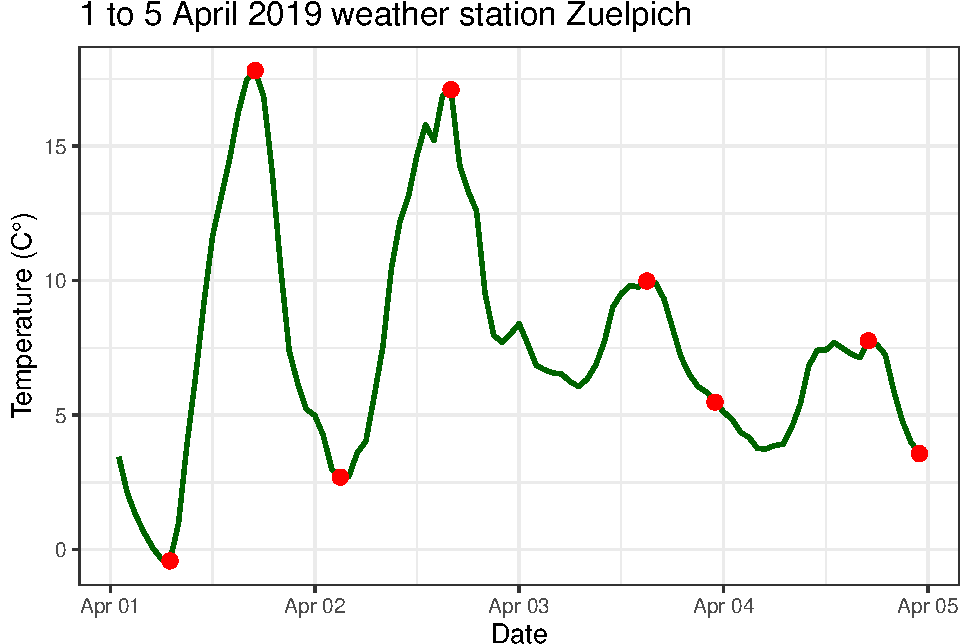
\includegraphics{Tree-Phenology_files/figure-latex/unnamed-chunk-23-1.pdf}

\begin{quote}
First, the dataset \texttt{ZU\_weather} must be created. The columns \texttt{DATE}, \texttt{Year}, \texttt{Month}, \texttt{Day}, \texttt{Tcontinue}, and \texttt{Temp\_inter} are created. The \texttt{Temp\_inter} column contains temperature data with large gaps that must be interpolated between.
\end{quote}

\begin{Shaded}
\begin{Highlighting}[]
\NormalTok{ZU_weather =}\StringTok{ }\KeywordTok{data.frame}\NormalTok{(}
  \DataTypeTok{DATE =}\NormalTok{ zuelpich_april[, }\DecValTok{4}\NormalTok{],}
  \DataTypeTok{Year =} \KeywordTok{as.numeric}\NormalTok{(}\KeywordTok{substr}\NormalTok{(zuelpich_april[, }\DecValTok{4}\NormalTok{], }\DecValTok{1}\NormalTok{, }\DecValTok{4}\NormalTok{)),}
  \DataTypeTok{Month =} \KeywordTok{as.numeric}\NormalTok{(}\KeywordTok{substr}\NormalTok{(zuelpich_april[, }\DecValTok{4}\NormalTok{], }\DecValTok{6}\NormalTok{, }\DecValTok{7}\NormalTok{)),}
  \DataTypeTok{Day =} \KeywordTok{as.numeric}\NormalTok{(}\KeywordTok{substr}\NormalTok{(zuelpich_april[, }\DecValTok{4}\NormalTok{], }\DecValTok{9}\NormalTok{, }\DecValTok{10}\NormalTok{)),}
  \DataTypeTok{Tcontinue =}\NormalTok{ zuelpich_april[, }\DecValTok{2}\NormalTok{],}
  \DataTypeTok{Temp_inter =}\NormalTok{ zuelpich_april[, }\DecValTok{6}\NormalTok{]}
\NormalTok{)}

\KeywordTok{kable}\NormalTok{(ZU_weather[}\DecValTok{1}\OperatorTok{:}\DecValTok{8}\NormalTok{,])}\OperatorTok\StringTok{ }
\StringTok{        }\KeywordTok{kable_styling}\NormalTok{(}\StringTok{"striped"}\NormalTok{, }\DataTypeTok{position =} \StringTok{"left"}\NormalTok{, }\DataTypeTok{font_size =} \DecValTok{10}\NormalTok{)}\OperatorTok
\StringTok{      }\KeywordTok{scroll_box}\NormalTok{(}\DataTypeTok{width =} \StringTok{"100%"}\NormalTok{)}
\end{Highlighting}
\end{Shaded}

\begingroup\fontsize{10}{12}\selectfont

\begin{tabular}{l|r|r|r|r|r}
\hline
DATE & Year & Month & Day & Tcontinue & Temp\_inter\\
\hline
2019-04-01 01:00:00 & 2019 & 4 & 1 & 3.4350000 & NA\\
\hline
2019-04-01 02:00:00 & 2019 & 4 & 1 & 2.0900000 & NA\\
\hline
2019-04-01 03:00:00 & 2019 & 4 & 1 & 1.2616667 & NA\\
\hline
2019-04-01 04:00:00 & 2019 & 4 & 1 & 0.6150000 & NA\\
\hline
2019-04-01 05:00:00 & 2019 & 4 & 1 & 0.0583333 & NA\\
\hline
2019-04-01 06:00:00 & 2019 & 4 & 1 & -0.3566667 & NA\\
\hline
2019-04-01 07:00:00 & 2019 & 4 & 1 & -0.4200000 & -0.42\\
\hline
2019-04-01 08:00:00 & 2019 & 4 & 1 & 0.9666667 & NA\\
\hline
\end{tabular}
\endgroup{}

\begin{quote}
The next step is to use the \texttt{interpolate\_gaps()} function to calculate the missing temperatures between \texttt{Tmax} and \texttt{Tmin}. The function \texttt{interpolate\_gaps()} returns a list with two entries. The first entry of the list contains the interpolated values, which can be accessed using \texttt{\$interp} or \texttt{{[}{[}1{]}{]}}. The second entry, \texttt{\$missing}, gives information on whether a value needs to be interpolated or if a real value is present. The function \texttt{interpolate\_gaps()} linearly interpolates between gaps in the temperature records. The interpolated values are written directly to the Temp\_inter column using the first list entry created by the \texttt{interpolate\_gaps()} function.
\end{quote}

\begin{Shaded}
\begin{Highlighting}[]
\CommentTok{# interpolate between gaps in coloum Temp_inter }
\NormalTok{ZU_weather}\OperatorTok{$}\NormalTok{Temp_inter <-}\StringTok{ }\KeywordTok{interpolate_gaps}\NormalTok{(ZU_weather}\OperatorTok{$}\NormalTok{Temp_inter)[[}\DecValTok{1}\NormalTok{]]}

\CommentTok{# have a look at the first 10 entries}
\KeywordTok{kable}\NormalTok{(ZU_weather[}\DecValTok{1}\OperatorTok{:}\DecValTok{10}\NormalTok{, ]) }\OperatorTok\StringTok{ }
\StringTok{        }\KeywordTok{kable_styling}\NormalTok{(}\StringTok{"striped"}\NormalTok{, }\DataTypeTok{position =} \StringTok{"left"}\NormalTok{, }\DataTypeTok{font_size =} \DecValTok{10}\NormalTok{)}\OperatorTok
\StringTok{        }\KeywordTok{scroll_box}\NormalTok{(}\DataTypeTok{width =} \StringTok{"100%"}\NormalTok{)}
\end{Highlighting}
\end{Shaded}

\begingroup\fontsize{10}{12}\selectfont

\begin{tabular}{l|r|r|r|r|r}
\hline
DATE & Year & Month & Day & Tcontinue & Temp\_inter\\
\hline
2019-04-01 01:00:00 & 2019 & 4 & 1 & 3.4350000 & -0.420\\
\hline
2019-04-01 02:00:00 & 2019 & 4 & 1 & 2.0900000 & -0.420\\
\hline
2019-04-01 03:00:00 & 2019 & 4 & 1 & 1.2616667 & -0.420\\
\hline
2019-04-01 04:00:00 & 2019 & 4 & 1 & 0.6150000 & -0.420\\
\hline
2019-04-01 05:00:00 & 2019 & 4 & 1 & 0.0583333 & -0.420\\
\hline
2019-04-01 06:00:00 & 2019 & 4 & 1 & -0.3566667 & -0.420\\
\hline
2019-04-01 07:00:00 & 2019 & 4 & 1 & -0.4200000 & -0.420\\
\hline
2019-04-01 08:00:00 & 2019 & 4 & 1 & 0.9666667 & 1.403\\
\hline
2019-04-01 09:00:00 & 2019 & 4 & 1 & 3.9333334 & 3.226\\
\hline
2019-04-01 10:00:00 & 2019 & 4 & 1 & 6.4183333 & 5.049\\
\hline
\end{tabular}
\endgroup{}

\begin{quote}
Thus, all gaps in the column \texttt{Temp\_inter} are filled by linear interpolation. The interpolation is performed between the gaps.

The non-linear interpolation method considers the sun's position at the respective location in the interpolation. In addition, the \texttt{stack\_hourly\_temps()} function requires a dataset as input that only contains \texttt{Tmax} and \texttt{Tmin} values. In this example, this dataset is called \texttt{ZU\_weather\_min\_max} and consists of five columns: \texttt{Year}, \texttt{Month}, \texttt{Day}, \texttt{Tmax}, and \texttt{Tmin}.
\end{quote}

\begin{Shaded}
\begin{Highlighting}[]
\CommentTok{# create dataframe for non-linear interpolation}
\NormalTok{ZU_weather_min_max =}\StringTok{ }\KeywordTok{data.frame}\NormalTok{(}
  \DataTypeTok{Year =} \KeywordTok{as.numeric}\NormalTok{(}\KeywordTok{substr}\NormalTok{(Zuelpich_min_max[, }\DecValTok{2}\NormalTok{], }\DecValTok{1}\NormalTok{, }\DecValTok{4}\NormalTok{)),}
  \DataTypeTok{Month =} \KeywordTok{as.numeric}\NormalTok{(}\KeywordTok{substr}\NormalTok{(Zuelpich_min_max[, }\DecValTok{2}\NormalTok{], }\DecValTok{6}\NormalTok{, }\DecValTok{7}\NormalTok{)),}
  \DataTypeTok{Day =} \KeywordTok{as.numeric}\NormalTok{(}\KeywordTok{substr}\NormalTok{(Zuelpich_min_max[, }\DecValTok{2}\NormalTok{], }\DecValTok{9}\NormalTok{, }\DecValTok{10}\NormalTok{)),}
  \DataTypeTok{Tmax =}\NormalTok{ final[, }\DecValTok{3}\NormalTok{],}
  \DataTypeTok{Tmin =}\NormalTok{ final[, }\DecValTok{4}\NormalTok{]}
\NormalTok{)}
\KeywordTok{kable}\NormalTok{(ZU_weather_min_max[}\DecValTok{1}\OperatorTok{:}\DecValTok{10}\NormalTok{,])}\OperatorTok
\StringTok{      }\KeywordTok{kable_styling}\NormalTok{(}\StringTok{"striped"}\NormalTok{, }\DataTypeTok{position =} \StringTok{"left"}\NormalTok{, }\DataTypeTok{font_size =} \DecValTok{10}\NormalTok{)}\OperatorTok
\StringTok{      }\KeywordTok{scroll_box}\NormalTok{(}\DataTypeTok{width =} \StringTok{"100%"}\NormalTok{)}
\end{Highlighting}
\end{Shaded}

\begingroup\fontsize{10}{12}\selectfont

\begin{tabular}{r|r|r|r|r}
\hline
Year & Month & Day & Tmax & Tmin\\
\hline
2019 & 2 & 2 & 17.810000 & -0.420000\\
\hline
2019 & 2 & 3 & 17.096667 & 2.693333\\
\hline
2019 & 2 & 4 & 9.983333 & 5.481667\\
\hline
2019 & 2 & 5 & 7.763333 & 3.566667\\
\hline
2019 & 2 & 6 & 17.810000 & -0.420000\\
\hline
2019 & 2 & 7 & 17.096667 & 2.693333\\
\hline
2019 & 2 & 8 & 9.983333 & 5.481667\\
\hline
2019 & 2 & 9 & 7.763333 & 3.566667\\
\hline
2019 & 2 & 10 & 17.810000 & -0.420000\\
\hline
2019 & 2 & 11 & 17.096667 & 2.693333\\
\hline
\end{tabular}
\endgroup{}

\begin{quote}
The function \texttt{stack\_hourly\_temps()} can be passed the entire dataset \texttt{ZU\_weather\_min\_max}. This function sets the \texttt{Tmax} values to 6:00 PM and the Tmin values to 6:00 AM, without performing any interpolation between the times when the \texttt{Tmax} and \texttt{Tmin} values actually occurred. The resulting interpolation is written to a new dataset, \texttt{ZU\_hourly}. A new column called \texttt{DATE} is then created in this dataset to store the date, and the first row is removed due to an index shift.
\end{quote}

\begin{Shaded}
\begin{Highlighting}[]
\NormalTok{ZU_hourly =}\StringTok{ }\KeywordTok{stack_hourly_temps}\NormalTok{(ZU_weather_min_max, }\DataTypeTok{latitude =} \FloatTok{50.4}\NormalTok{)}

\NormalTok{ZU_hourly}\OperatorTok{$}\NormalTok{hourtemps[, }\StringTok{"DATE"}\NormalTok{] =}
\StringTok{  }\KeywordTok{ISOdate}\NormalTok{(}
\NormalTok{    ZU_hourly}\OperatorTok{$}\NormalTok{hourtemps}\OperatorTok{$}\NormalTok{Year,}
\NormalTok{    ZU_hourly}\OperatorTok{$}\NormalTok{hourtemps}\OperatorTok{$}\NormalTok{Month,}
\NormalTok{    ZU_hourly}\OperatorTok{$}\NormalTok{hourtemps}\OperatorTok{$}\NormalTok{Day,}
\NormalTok{    ZU_hourly}\OperatorTok{$}\NormalTok{hourtemps}\OperatorTok{$}\NormalTok{Hour}
\NormalTok{  )}

\NormalTok{ZU_hourly_mod =}\StringTok{ }\NormalTok{ZU_hourly[[}\DecValTok{1}\NormalTok{]][}\OperatorTok{-}\DecValTok{1}\NormalTok{, ]}

\KeywordTok{kable}\NormalTok{(ZU_hourly_mod[}\DecValTok{1}\OperatorTok{:}\DecValTok{10}\NormalTok{,])}\OperatorTok\StringTok{ }
\StringTok{      }\KeywordTok{kable_styling}\NormalTok{(}\StringTok{"striped"}\NormalTok{, }\DataTypeTok{position =} \StringTok{"left"}\NormalTok{, }\DataTypeTok{font_size =} \DecValTok{10}\NormalTok{)}\OperatorTok
\StringTok{      }\KeywordTok{scroll_box}\NormalTok{(}\DataTypeTok{width =} \StringTok{"100%"}\NormalTok{)}
\end{Highlighting}
\end{Shaded}

\begingroup\fontsize{10}{12}\selectfont

\begin{tabular}{l|r|r|r|r|r|r|r|r|l}
\hline
  & Year & Month & Day & Tmax & Tmin & JDay & Hour & Temp & DATE\\
\hline
609 & 2019 & 2 & 2 & 17.81 & -0.42 & 33 & 1 & -0.420000 & 2019-02-02 01:00:00\\
\hline
1217 & 2019 & 2 & 2 & 17.81 & -0.42 & 33 & 2 & -0.420000 & 2019-02-02 02:00:00\\
\hline
1825 & 2019 & 2 & 2 & 17.81 & -0.42 & 33 & 3 & -0.420000 & 2019-02-02 03:00:00\\
\hline
2433 & 2019 & 2 & 2 & 17.81 & -0.42 & 33 & 4 & -0.420000 & 2019-02-02 04:00:00\\
\hline
3041 & 2019 & 2 & 2 & 17.81 & -0.42 & 33 & 5 & -0.420000 & 2019-02-02 05:00:00\\
\hline
3649 & 2019 & 2 & 2 & 17.81 & -0.42 & 33 & 6 & -0.420000 & 2019-02-02 06:00:00\\
\hline
4257 & 2019 & 2 & 2 & 17.81 & -0.42 & 33 & 7 & -0.420000 & 2019-02-02 07:00:00\\
\hline
4865 & 2019 & 2 & 2 & 17.81 & -0.42 & 33 & 8 & 2.355706 & 2019-02-02 08:00:00\\
\hline
5473 & 2019 & 2 & 2 & 17.81 & -0.42 & 33 & 9 & 6.496980 & 2019-02-02 09:00:00\\
\hline
6081 & 2019 & 2 & 2 & 17.81 & -0.42 & 33 & 10 & 10.253744 & 2019-02-02 10:00:00\\
\hline
\end{tabular}
\endgroup{}

\begin{quote}
Finally, a dataset is generated containing the actual measured temperature data, as well as the interpolated values calculated using both linear and non-linear interpolation. The results can be effectively visualized in a plot.
\end{quote}

\begin{Shaded}
\begin{Highlighting}[]
\CommentTok{# final_df = data.frame(}
\CommentTok{#   DATE = zuelpich_april[, 4],}
\CommentTok{#   Measured_Temp = zuelpich_april[, 2],}
\CommentTok{#   Linear_Interp  = ZU_weather[, 6],}
\CommentTok{#   Non_Linear_Interp = ZU_hourly_mod[, 8]}
\CommentTok{# )}
\CommentTok{#write.csv(final_df, "weather_data/final_df_non_linear.csv")}

\CommentTok{# read final dataframe}
\NormalTok{final_df_m =}\StringTok{ }\KeywordTok{read.table}\NormalTok{(}\StringTok{"weather_data/final_df_non_linear.csv"}\NormalTok{,}
                        \DataTypeTok{header =} \OtherTok{TRUE}\NormalTok{,}
                        \DataTypeTok{sep =} \StringTok{","}\NormalTok{)}

\CommentTok{#remove index}
\NormalTok{final_df_mx =}\StringTok{ }\NormalTok{final_df_m[, }\DecValTok{-1}\NormalTok{]}

\CommentTok{#generate Date}
\NormalTok{final_df_mx}\OperatorTok{$}\NormalTok{DATE =}\StringTok{  }\KeywordTok{as.POSIXct}\NormalTok{(final_df_mx}\OperatorTok{$}\NormalTok{DATE)}

\CommentTok{#create pivot table}
\NormalTok{final_df_mod  =}\StringTok{ }\KeywordTok{pivot_longer}\NormalTok{(final_df_mx,}
                             \OperatorTok{-}\StringTok{"DATE"}\NormalTok{,}
                             \DataTypeTok{names_to =} \StringTok{"Method"}\NormalTok{,}
                             \DataTypeTok{values_to =} \StringTok{"Temperature"}\NormalTok{)}

\CommentTok{#plot final result and compare methods}
\KeywordTok{ggplot}\NormalTok{(}\DataTypeTok{data =}\NormalTok{ final_df_mod, }\KeywordTok{aes}\NormalTok{(}\DataTypeTok{x =}\NormalTok{ DATE, }\DataTypeTok{y =}\NormalTok{ Temperature}
\NormalTok{                                , }\DataTypeTok{colour =}\NormalTok{ Method)) }\OperatorTok{+}
\StringTok{  }\KeywordTok{geom_line}\NormalTok{(}\DataTypeTok{lwd =} \FloatTok{1.3}\NormalTok{) }\OperatorTok{+}
\StringTok{  }\KeywordTok{labs}\NormalTok{(}\DataTypeTok{x =} \StringTok{"Date"}\NormalTok{, }\DataTypeTok{y =} \StringTok{"Temperature (C°)"}\NormalTok{) }\OperatorTok{+}
\StringTok{  }\KeywordTok{ggtitle}\NormalTok{(}\StringTok{"1 to 5 April 2019  Zuelpich"}\NormalTok{) }\OperatorTok{+}
\StringTok{  }\KeywordTok{scale_color_manual}\NormalTok{(}\DataTypeTok{values =} \KeywordTok{c}\NormalTok{(}\StringTok{"red"}\NormalTok{, }\StringTok{"darkgreen"}\NormalTok{, }\StringTok{"darkblue"}\NormalTok{)) }\OperatorTok{+}
\StringTok{  }\CommentTok{#facet_wrap(vars(Method)) +}
\StringTok{  }\KeywordTok{theme_bw}\NormalTok{(}\DataTypeTok{base_size =} \DecValTok{15}\NormalTok{)}
\end{Highlighting}
\end{Shaded}

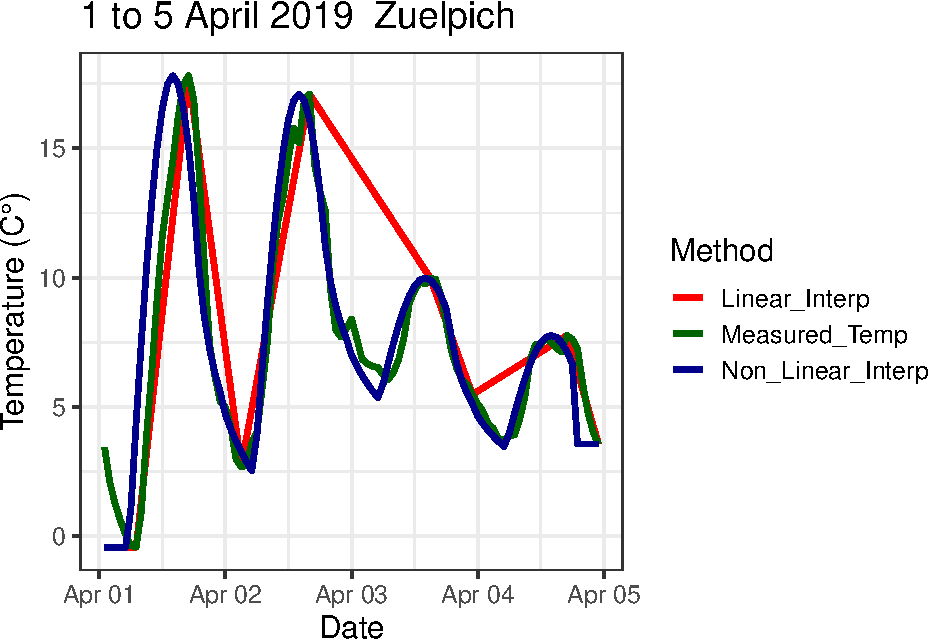
\includegraphics{Tree-Phenology_files/figure-latex/unnamed-chunk-28-1.pdf}

\hypertarget{getting-temperature-data}{%
\chapter{Getting temperature data}\label{getting-temperature-data}}

\hypertarget{task-1-5}{%
\section{Task 1}\label{task-1-5}}

\textbf{Choose a location of interest and find the 25 closest weather stations using the handle\_gsod function}

\begin{quote}
I have decided to conduct a phonology analysis at a location in Poland. The city of Glogau, situated on the banks of the Oder, was chosen as the starting point. For more information about the location, the following website can be visited \href{https://de.wikipedia.org/wiki/G\%C5\%82og\%C3\%B3w}{here}.
The climate at the location is relatively similar to Bonn, although the climate is generally more continental, which can be reflected in colder winters and drier, slightly warmer summers.
Here is a picture of a typical landscape in Lower Silesia in Poland.
\end{quote}

\begin{quote}
Beautiful Glogau City
\end{quote}

\begin{quote}
Ok, here really beautiful old city of Glogau
\end{quote}

\begin{Shaded}
\begin{Highlighting}[]
\CommentTok{# station_list_poland = handle_gsod(action="list_stations",}
\CommentTok{#                            location=c(16.5,51.39),}
\CommentTok{#                            time_interval=c(1990,2020))}
\CommentTok{# kable(station_list_poland[1:10,]) %>% kable_styling("striped", position = "left", font_size = 10)}

\CommentTok{# write.csv(station_list_poland,"weather_data/Poland_station_list.csv",row.names=FALSE)}

\NormalTok{list_poland_weather =}\StringTok{ }\KeywordTok{read.table}\NormalTok{(}\StringTok{"weather_data/Poland_station_list.csv"}\NormalTok{, }\DataTypeTok{header =} \OtherTok{TRUE}\NormalTok{, }\DataTypeTok{sep=}\StringTok{","}\NormalTok{)}
\KeywordTok{kable}\NormalTok{(list_poland_weather[}\DecValTok{1}\OperatorTok{:}\DecValTok{10}\NormalTok{,], }\DataTypeTok{caption =} \StringTok{"Station List"}\NormalTok{) }\OperatorTok\StringTok{ }
\StringTok{  }\KeywordTok{kable_styling}\NormalTok{(}\StringTok{"striped"}\NormalTok{, }\DataTypeTok{position =} \StringTok{"left"}\NormalTok{, }\DataTypeTok{font_size =} \DecValTok{10}\NormalTok{)}\OperatorTok
\StringTok{  }\KeywordTok{scroll_box}\NormalTok{(}\DataTypeTok{width =} \StringTok{"100%"}\NormalTok{)}
\end{Highlighting}
\end{Shaded}

\begin{table}

\caption{\label{tab:unnamed-chunk-29}Station List}
\fontsize{10}{12}\selectfont
\begin{tabular}[t]{l|l|l|r|r|r|r|r|r|r}
\hline
chillR\_code & STATION.NAME & CTRY & Lat & Long & BEGIN & END & distance & Overlap\_years & Perc\_interval\_covered\\
\hline
124170\_99999 & LUBIN MIASTO & PL & 51.417 & 16.200 & 19390810 & 19411231 & 21.09 & 0.00 & 0.00\\
\hline
124150\_99999 & LEGNICA & PL & 51.200 & 16.200 & 19370401 & 20221110 & 29.74 & 31.00 & 100.00\\
\hline
124250\_99999 & WROCLAW I & PL & 51.117 & 16.883 & 19280101 & 20220614 & 40.47 & 31.00 & 100.00\\
\hline
124240\_99999 & STRACHOWICE & PL & 51.103 & 16.886 & 19390102 & 20221110 & 41.78 & 31.00 & 100.00\\
\hline
124280\_99999 & WROCLAW/STRACHOWICE & PL & 51.100 & 16.883 & 20020601 & 20220901 & 41.91 & 18.59 & 59.95\\
\hline
124160\_99999 & WSCHOWA & PL & 51.800 & 16.317 & 19360102 & 19420630 & 47.35 & 0.00 & 0.00\\
\hline
124180\_99999 & LESZNO & PL & 51.833 & 16.533 & 19730101 & 20211212 & 49.34 & 31.00 & 100.00\\
\hline
125010\_99999 & MIROSLAWICE & PL & 50.950 & 16.767 & 19390901 & 19420628 & 52.39 & 0.00 & 0.00\\
\hline
125230\_99999 & SWIDNICA & PL & 50.850 & 16.483 & 19410114 & 19431231 & 60.09 & 0.00 & 0.00\\
\hline
125220\_99999 & SLEZA & PL & 50.867 & 16.717 & 19400414 & 19420630 & 60.13 & 0.00 & 0.00\\
\hline
\end{tabular}
\end{table}

\hypertarget{task-2-4}{%
\section{Task 2}\label{task-2-4}}

\textbf{Download weather data for the most promising station on the list}

\begin{quote}
The most promising station for obtaining continuous weather recording is represented by the weather station in Leszno, located approximately 50 kilometers (by air) from Glogau. This location is listed as the seventh entry in the ``Station List'' table.

To avoid constantly loading the weather data, it is stored in the \texttt{weather\_poland\_leszno} variable. The file is then saved as a CSV and read in using the \texttt{read.table()} function.
\end{quote}

\begin{Shaded}
\begin{Highlighting}[]
\CommentTok{# weather_poland_leszno <- handle_gsod(}
\CommentTok{#   action = "download_weather",}
\CommentTok{#   location = station_list_poland$chillR_code[7],}
\CommentTok{#   time_interval = c(1990, 2020))}


\CommentTok{# kable(weather_poland_leszno[[1]][[2]][1:10, ]) %>%}
\CommentTok{#   kable_styling("striped", position = "left", font_size = 10)}

\CommentTok{#write.csv(weather_poland_leszno[[1]][[2]],"weather_data/Poland_leszno_weather.csv",row.names=FALSE)}

\NormalTok{weather_poland_leszno_place =}\StringTok{ }
\StringTok{  }\KeywordTok{read.table}\NormalTok{(}\StringTok{"weather_data/Poland_leszno_weather.csv"}\NormalTok{, }\DataTypeTok{header =} \OtherTok{TRUE}\NormalTok{, }\DataTypeTok{sep=}\StringTok{","}\NormalTok{)}

\KeywordTok{kable}\NormalTok{(weather_poland_leszno_place[}\DecValTok{1}\OperatorTok{:}\DecValTok{10}\NormalTok{, ], }\DataTypeTok{caption =} \StringTok{"Weather Data Leszno "}\NormalTok{) }\OperatorTok
\StringTok{   }\KeywordTok{kable_styling}\NormalTok{(}\StringTok{"striped"}\NormalTok{, }\DataTypeTok{position =} \StringTok{"left"}\NormalTok{, }\DataTypeTok{font_size =} \DecValTok{10}\NormalTok{)}\OperatorTok
\StringTok{   }\KeywordTok{scroll_box}\NormalTok{(}\DataTypeTok{width =} \StringTok{"100%"}\NormalTok{)}
\end{Highlighting}
\end{Shaded}

\begin{table}

\caption{\label{tab:unnamed-chunk-30}Weather Data Leszno }
\fontsize{10}{12}\selectfont
\begin{tabular}[t]{l|r|r|r|r|r|r|r|r|r|r|r|r|r|r|r|r|r|r|l|r|l|r|l|r|l|r|r|r|r|r}
\hline
DATE & STN... & WBAN & YEAR & MONTH & DAY & TEMP & Count1 & DEWP & Count2 & SLP & Count3 & STP & Count4 & VISIB & Count5 & WDSP & Count6 & MXSPD & GUST & MAX & MaxFlag & MIN & MinFlag & PRCP & PrcpFlag & SNDP & FRSHTT & Year & Month & Day\\
\hline
1990-01-01 12:00:00 & 124180 & 99999 & 1990 & 1 & 1 & -1.1111111 & 7 & 28.6 & 7 & 1022.2 & 7 & NA & 0 & 1.1 & 7 & 1.9 & 7 & 3.9 & NA & -0.6111111 &  & -2.000000 &  & 0.000 & E & NA & 1000 & 1990 & 1 & 1\\
\hline
1990-01-02 12:00:00 & 124180 & 99999 & 1990 & 1 & 2 & -1.7222222 & 8 & 25.9 & 8 & 1023.3 & 8 & NA & 0 & 1.5 & 8 & 3.2 & 8 & 5.8 & NA & -1.2777778 &  & -2.111111 & * & 0.000 & F & NA & 1000 & 1990 & 1 & 2\\
\hline
1990-01-03 12:00:00 & 124180 & 99999 & 1990 & 1 & 3 & -1.7777778 & 7 & 25.6 & 7 & 1028.2 & 7 & NA & 0 & 1.9 & 7 & 3.6 & 7 & 5.8 & NA & -0.7777778 &  & -2.611111 &  & 0.000 & F & NA & 1000 & 1990 & 1 & 3\\
\hline
1990-01-04 12:00:00 & 124180 & 99999 & 1990 & 1 & 4 & -2.4444444 & 7 & 22.5 & 7 & 1029.0 & 7 & NA & 0 & 2.9 & 7 & 6.1 & 7 & 11.7 & NA & -0.7777778 &  & -5.277778 & * & 0.000 & C & NA & 0 & 1990 & 1 & 4\\
\hline
1990-01-05 12:00:00 & 124180 & 99999 & 1990 & 1 & 5 & -2.3888889 & 7 & 22.6 & 7 & 1026.5 & 6 & NA & 0 & 2.2 & 7 & 4.4 & 7 & 7.8 & NA & -0.3888889 &  & -7.722222 &  & 0.000 & D & NA & 0 & 1990 & 1 & 5\\
\hline
1990-01-06 12:00:00 & 124180 & 99999 & 1990 & 1 & 6 & -4.7777778 & 7 & 21.3 & 7 & 1032.6 & 6 & NA & 0 & 1.4 & 7 & 2.5 & 7 & 3.9 & NA & 0.0000000 &  & -7.000000 &  & 0.000 & C & NA & 0 & 1990 & 1 & 6\\
\hline
1990-01-07 12:00:00 & 124180 & 99999 & 1990 & 1 & 7 & -7.3333333 & 8 & 15.4 & 8 & 1033.4 & 8 & NA & 0 & 1.1 & 8 & 3.4 & 8 & 5.8 & NA & -2.7222222 & * & -11.611111 &  & 0.000 & D & NA & 0 & 1990 & 1 & 7\\
\hline
1990-01-08 12:00:00 & 124180 & 99999 & 1990 & 1 & 8 & -4.5555556 & 8 & 18.0 & 8 & 1033.4 & 8 & NA & 0 & 1.6 & 8 & 4.6 & 8 & 7.8 & NA & 1.1111111 &  & -10.500000 &  & 0.000 & D & NA & 0 & 1990 & 1 & 8\\
\hline
1990-01-09 12:00:00 & 124180 & 99999 & 1990 & 1 & 9 & 0.8333333 & 6 & 33.1 & 6 & 1033.8 & 6 & NA & 0 & 0.7 & 6 & 6.6 & 5 & 7.8 & NA & 2.1111111 & * & -1.777778 &  & 0.000 & E & NA & 110000 & 1990 & 1 & 9\\
\hline
1990-01-10 12:00:00 & 124180 & 99999 & 1990 & 1 & 10 & 2.7222222 & 7 & 36.3 & 7 & 1030.9 & 6 & NA & 0 & 1.1 & 7 & 6.9 & 7 & 9.7 & NA & 3.2777778 & * & 1.500000 &  & 0.254 & F & NA & 110000 & 1990 & 1 & 10\\
\hline
\end{tabular}
\end{table}

\hypertarget{task-3-2}{%
\section{Task 3}\label{task-3-2}}

\textbf{Convert the weather data into chillR format}

\begin{Shaded}
\begin{Highlighting}[]
\CommentTok{# weather_pl <- weather_poland_leszno$LESZNO[[2]]}
\CommentTok{# cleaned_weather_pl <- handle_gsod(weather_pl)}

\CommentTok{# kable(cleaned_weather_pl[1:20,]) %>%}
\CommentTok{#   kable_styling("striped", position = "left", font_size = 10)}

\CommentTok{#write.csv(cleaned_weather_pl,"weather_data/Poland_leszno_chillR_weather.csv",row.names=FALSE)}

\NormalTok{cleaned_weather_pl_leszno =}\StringTok{ }\KeywordTok{read.table}\NormalTok{(}\StringTok{"weather_data/Poland_leszno_chillR_weather.csv"}\NormalTok{, }\DataTypeTok{header =} \OtherTok{TRUE}\NormalTok{, }\DataTypeTok{sep =} \StringTok{","}\NormalTok{)}

\KeywordTok{kable}\NormalTok{(cleaned_weather_pl_leszno[}\DecValTok{1}\OperatorTok{:}\DecValTok{10}\NormalTok{, ], }\DataTypeTok{caption =} \StringTok{"Cleaned Weather Data Leszno"}\NormalTok{) }\OperatorTok
\StringTok{   }\KeywordTok{kable_styling}\NormalTok{(}\StringTok{"striped"}\NormalTok{, }\DataTypeTok{position =} \StringTok{"left"}\NormalTok{, }\DataTypeTok{font_size =} \DecValTok{10}\NormalTok{)}
\end{Highlighting}
\end{Shaded}

\begin{table}

\caption{\label{tab:unnamed-chunk-31}Cleaned Weather Data Leszno}
\fontsize{10}{12}\selectfont
\begin{tabular}[t]{l|r|r|r|r|r|r|r}
\hline
DATE & Year & Month & Day & Tmin & Tmax & Tmean & Prec\\
\hline
1990-01-01 12:00:00 & 1990 & 1 & 1 & -2.000000 & -0.6111111 & -1.1111111 & 0.000\\
\hline
1990-01-02 12:00:00 & 1990 & 1 & 2 & -2.111111 & -1.2777778 & -1.7222222 & 0.000\\
\hline
1990-01-03 12:00:00 & 1990 & 1 & 3 & -2.611111 & -0.7777778 & -1.7777778 & 0.000\\
\hline
1990-01-04 12:00:00 & 1990 & 1 & 4 & -5.277778 & -0.7777778 & -2.4444444 & 0.000\\
\hline
1990-01-05 12:00:00 & 1990 & 1 & 5 & -7.722222 & -0.3888889 & -2.3888889 & 0.000\\
\hline
1990-01-06 12:00:00 & 1990 & 1 & 6 & -7.000000 & 0.0000000 & -4.7777778 & 0.000\\
\hline
1990-01-07 12:00:00 & 1990 & 1 & 7 & -11.611111 & -2.7222222 & -7.3333333 & 0.000\\
\hline
1990-01-08 12:00:00 & 1990 & 1 & 8 & -10.500000 & 1.1111111 & -4.5555556 & 0.000\\
\hline
1990-01-09 12:00:00 & 1990 & 1 & 9 & -1.777778 & 2.1111111 & 0.8333333 & 0.000\\
\hline
1990-01-10 12:00:00 & 1990 & 1 & 10 & 1.500000 & 3.2777778 & 2.7222222 & 0.254\\
\hline
\end{tabular}
\end{table}

\hypertarget{filling-gaps-in-temperature-records}{%
\chapter{Filling gaps in temperature records}\label{filling-gaps-in-temperature-records}}

\hypertarget{task-1-6}{%
\section{Task 1}\label{task-1-6}}

\textbf{Use chillR functions to find out how many gaps you have in this dataset (even if you have none, please still follow all further steps)}

\begin{Shaded}
\begin{Highlighting}[]
\NormalTok{Leszno =}\StringTok{ }\KeywordTok{read.csv}\NormalTok{(}\StringTok{"weather_data/Poland_leszno_chillR_weather.csv"}\NormalTok{)}

\CommentTok{# detected many gaps }
\NormalTok{Leszno_QC =}\StringTok{ }\KeywordTok{fix_weather}\NormalTok{(Leszno)}\OperatorTok{$}\NormalTok{QC}

\KeywordTok{kable}\NormalTok{(Leszno_QC, }\DataTypeTok{caption =} \StringTok{"Quality Check  for Data Leszno "}\NormalTok{) }\OperatorTok
\StringTok{  }\KeywordTok{kable_styling}\NormalTok{(}\StringTok{"striped"}\NormalTok{, }\DataTypeTok{position =} \StringTok{"left"}\NormalTok{, }\DataTypeTok{font_size =} \DecValTok{10}\NormalTok{) }\OperatorTok
\StringTok{  }\KeywordTok{scroll_box}\NormalTok{(}\DataTypeTok{width =} \StringTok{"100%"}\NormalTok{)}
\end{Highlighting}
\end{Shaded}

\begin{table}

\caption{\label{tab:unnamed-chunk-32}Quality Check  for Data Leszno }
\fontsize{10}{12}\selectfont
\begin{tabular}[t]{l|r|r|r|r|r|r|r}
\hline
Season & End\_year & Season\_days & Data\_days & Missing\_Tmin & Missing\_Tmax & Incomplete\_days & Perc\_complete\\
\hline
1989/1990 & 1990 & 365 & 365 & 1 & 1 & 1 & 99.7\\
\hline
1990/1991 & 1991 & 365 & 365 & 26 & 26 & 26 & 92.9\\
\hline
1991/1992 & 1992 & 366 & 366 & 284 & 284 & 284 & 22.4\\
\hline
1992/1993 & 1993 & 365 & 365 & 140 & 140 & 140 & 61.6\\
\hline
1993/1994 & 1994 & 365 & 365 & 57 & 57 & 57 & 84.4\\
\hline
1994/1995 & 1995 & 365 & 365 & 4 & 4 & 4 & 98.9\\
\hline
1995/1996 & 1996 & 366 & 366 & 5 & 5 & 5 & 98.6\\
\hline
1996/1997 & 1997 & 365 & 365 & 75 & 75 & 75 & 79.5\\
\hline
1997/1998 & 1998 & 365 & 365 & 140 & 140 & 140 & 61.6\\
\hline
1998/1999 & 1999 & 365 & 365 & 39 & 39 & 39 & 89.3\\
\hline
1999/2000 & 2000 & 366 & 366 & 1 & 1 & 1 & 99.7\\
\hline
2000/2001 & 2001 & 365 & 365 & 23 & 23 & 23 & 93.7\\
\hline
2001/2002 & 2002 & 365 & 365 & 4 & 4 & 4 & 98.9\\
\hline
2002/2003 & 2003 & 365 & 365 & 1 & 1 & 1 & 99.7\\
\hline
2003/2004 & 2004 & 366 & 366 & 2 & 2 & 2 & 99.5\\
\hline
2004/2005 & 2005 & 365 & 365 & 365 & 365 & 365 & 0.0\\
\hline
2005/2006 & 2006 & 365 & 365 & 365 & 365 & 365 & 0.0\\
\hline
2006/2007 & 2007 & 365 & 365 & 365 & 365 & 365 & 0.0\\
\hline
2007/2008 & 2008 & 366 & 366 & 366 & 366 & 366 & 0.0\\
\hline
2008/2009 & 2009 & 365 & 365 & 365 & 365 & 365 & 0.0\\
\hline
2009/2010 & 2010 & 365 & 365 & 365 & 365 & 365 & 0.0\\
\hline
2010/2011 & 2011 & 365 & 365 & 365 & 365 & 365 & 0.0\\
\hline
2011/2012 & 2012 & 366 & 366 & 366 & 366 & 366 & 0.0\\
\hline
2012/2013 & 2013 & 365 & 365 & 365 & 365 & 365 & 0.0\\
\hline
2013/2014 & 2014 & 365 & 365 & 365 & 365 & 365 & 0.0\\
\hline
2014/2015 & 2015 & 365 & 365 & 365 & 365 & 365 & 0.0\\
\hline
2015/2016 & 2016 & 366 & 366 & 366 & 366 & 366 & 0.0\\
\hline
2016/2017 & 2017 & 365 & 365 & 365 & 365 & 365 & 0.0\\
\hline
2017/2018 & 2018 & 365 & 365 & 365 & 365 & 365 & 0.0\\
\hline
2018/2019 & 2019 & 365 & 365 & 365 & 365 & 365 & 0.0\\
\hline
2019/2020 & 2020 & 366 & 366 & 366 & 366 & 366 & 0.0\\
\hline
\end{tabular}
\end{table}

\begin{quote}
Upon closer examination, the seemingly promising location of Leszno exhibits many gaps in temperature data, particularly after 2005. These gaps must be filled with temperature data from neighboring stations.
\end{quote}

\hypertarget{task-2-5}{%
\section{Task 2}\label{task-2-5}}

\textbf{Create a list of the 25 closest weather stations using the handle\_gsod function}

\begin{Shaded}
\begin{Highlighting}[]
\CommentTok{# station_list_close_to_leszno<-}
\CommentTok{#   handle_gsod(action="list_stations",location=c(16.57,51.85),time_interval=c(1990,2020))}

\CommentTok{# write.csv(station_list_close_to_leszno,"station_list_close_to_leszno.csv" )}

\NormalTok{station_list_close_to_leszno =}\StringTok{ }\KeywordTok{read.csv}\NormalTok{(}\StringTok{"station_list_close_to_leszno.csv"}\NormalTok{)}

\KeywordTok{kable}\NormalTok{(station_list_close_to_leszno[}\DecValTok{1}\OperatorTok{:}\DecValTok{10}\NormalTok{,], }
      \DataTypeTok{caption=}\StringTok{"List of GSOD weather stations close to Leszno"}\NormalTok{)}\OperatorTok
\StringTok{  }\KeywordTok{kable_styling}\NormalTok{(}\StringTok{"striped"}\NormalTok{, }\DataTypeTok{position =} \StringTok{"left"}\NormalTok{, }\DataTypeTok{font_size =} \DecValTok{10}\NormalTok{) }\OperatorTok
\StringTok{  }\KeywordTok{scroll_box}\NormalTok{(}\DataTypeTok{width =} \StringTok{"100%"}\NormalTok{)}
\end{Highlighting}
\end{Shaded}

\begin{table}

\caption{\label{tab:unnamed-chunk-33}List of GSOD weather stations close to Leszno}
\fontsize{10}{12}\selectfont
\begin{tabular}[t]{r|l|l|l|r|r|r|r|r|r|r}
\hline
X & chillR\_code & STATION.NAME & CTRY & Lat & Long & BEGIN & END & distance & Overlap\_years & Perc\_interval\_covered\\
\hline
4162 & 124180\_99999 & LESZNO & PL & 51.833 & 16.533 & 19730101 & 20211212 & 3.17 & 31.00 & 100.00\\
\hline
4160 & 124160\_99999 & WSCHOWA & PL & 51.800 & 16.317 & 19360102 & 19420630 & 18.31 & 0.00 & 0.00\\
\hline
4161 & 124170\_99999 & LUBIN MIASTO & PL & 51.417 & 16.200 & 19390810 & 19411231 & 54.56 & 0.00 & 0.00\\
\hline
4122 & 123260\_99999 & KRZESINY & PL & 52.332 & 16.966 & 20020601 & 20230103 & 60.11 & 18.59 & 59.95\\
\hline
4153 & 124030\_99999 & NOWE MIASTECZKO & PL & 51.683 & 15.733 & 19360102 & 19420630 & 60.70 & 0.00 & 0.00\\
\hline
4118 & 123120\_99999 & BABIMOST & PL & 52.139 & 15.799 & 20020603 & 20230103 & 61.96 & 18.58 & 59.94\\
\hline
4124 & 123300\_99999 & LAWICA & PL & 52.421 & 16.826 & 19310102 & 20230103 & 65.91 & 31.00 & 100.00\\
\hline
4163 & 124190\_99999 & JAROCIN & PL & 51.967 & 17.550 & 19391113 & 19420630 & 68.69 & 0.00 & 0.00\\
\hline
4150 & 124000\_99999 & ZIELONA GORA & PL & 51.933 & 15.533 & 19310101 & 20230103 & 71.99 & 31.00 & 100.00\\
\hline
4156 & 124060\_99999 & SZPROTAWA-WIECHLICE & PL & 51.561 & 15.585 & 19390815 & 20191108 & 75.30 & 29.85 & 96.30\\
\hline
\end{tabular}
\end{table}

\hypertarget{task-3-3}{%
\section{Task 3}\label{task-3-3}}

\textbf{Identify suitable weather stations for patching gaps}

\begin{quote}
After reviewing the nearest weather stations to the Leszno location, KRZESINY, BABIMOST and LAWICA stations were identified as suitable for filling in the gaps in temperature data. These stations are ranked 4th, 6th and 7th on the list.
\end{quote}

  \bibliography{book.bib,packages.bib}

\end{document}
